\documentclass[journal,twoside,web]{ieeecolor}
\usepackage{jsen}
\usepackage{cite}
\usepackage{amsmath,amssymb,amsfonts}
\usepackage{algpseudocode}
\usepackage{algorithm}
\usepackage{graphicx}
\usepackage{subcaption}
\usepackage{textcomp}
\usepackage{wrapfig}
\usepackage{xurl}
\usepackage{hyperref}
\usepackage[nolist]{acronym}
\usepackage{multirow}
\usepackage{booktabs}

\def\BibTeX{{\rm B\kern-.05em{\sc i\kern-.025em b}\kern-.08em
    T\kern-.1667em\lower.7ex\hbox{E}\kern-.125emX}}
\markboth{\journalname, VOL. XX, NO. XX, XXXX 2024}
{Author \MakeLowercase{\textit{et al.}}: Preparation of Papers for IEEE TRANSACTIONS and JOURNALS (May 2024)}
\definecolor{abstractbg}{rgb}{0.89804,0.94510,0.83137}
\setlength{\fboxrule}{0pt}
\setlength{\fboxsep}{0pt}


\begin{document}

\begin{acronym}
    \acro{YOLO}{You Look Only Once}
    \acro{PSD}{Platform Screen Door}
    \acro{CCTV}{Closed Circuit Television}
    % \acro{MS}{}
    \acro{MS COCO}{Microsoft Common Objects in Context}
    \acro{HAR}{Human Activity Recognition}
    \acro{ViT}{Vision Transformer}
    \acro{PASCAL}{pattern analysis, statistical modelling and computational learning}
    \acro{mAP}{mean Average Precision}
    \acro{AP}{Average Precision}
    \acro{IoU}{Intersection over Union}
    \acro{VOC}{Visual Object Classes}
    \acro{SD-Net}{Safe Door Network}
    \acro{PFL}{Parallel Feature Link}
    \acro{CNN}{Convolutional Neural Network}
    \acro{FCN}{Fully Convolutional Architecture}
    \acro{ELAN}{Extended Efficient Layer Aggregation Network}
    \acro{FLOPS}{Floating point Operations per second}
    \acro{RPN}{Region Proposal Network}
    \acro{BPR}{Best Possible Recall}
    \acro{GA}{Genetic Algorithm}
    \acro{IRB}{Institutional Review Board}
    \acro{fps}{frames per second}
    \acro{SGD}{Stochastic Gradient Descent}
    \acro{NMS}{Non-Maximum Suppression}
\end{acronym}

\title{SD-Net: An Efficient Object Detection Network for Proactive Subway Passenger Safety}

\author{
    Hee Jo, \IEEEmembership{Member, IEEE}, 
    Lisa Lim$^{*}$, \IEEEmembership{Member, IEEE},
    and Jo Woon Chong$^{*}$, \IEEEmembership{Member, IEEE}
    \thanks{* Corresponding authors: Lisa Lim and Jo Woon Chong}
    \thanks{This paragraph of the first footnote will contain the date on which you submitted your paper for review. It will also contain support information, including sponsor and financial support acknowledgment. For example, ``This work was supported in part by the U.S. Department of Commerce under Grant BS123456.'' }
    \thanks{Hee Jo is with the Department of Electrical and Computer Engineering, Sungkyunkwan University, Suwon 16419, Republic of Korea.}
    \thanks{Lisa Lim is with the Department of Civil and Environmental Engineering, Korea Advanced Institute of Science and Technology, Daejeon 34141, Republic of Korea (e-mail: lisalim@kaist.ac.kr).}
    \thanks{Jo Woon Chong is with the School of Electronic and Electrical Engineering, Sungkyunkwan University, Sungkyunkwan University, Suwon 16419, Republic of Korea (e-mail: jwchong@skku.edu).}
}

\IEEEtitleabstractindextext{%
    \fcolorbox{abstractbg}{abstractbg}{%
        \begin{minipage}{\textwidth}%
        \begin{wrapfigure}[12]{r}{3in}%
        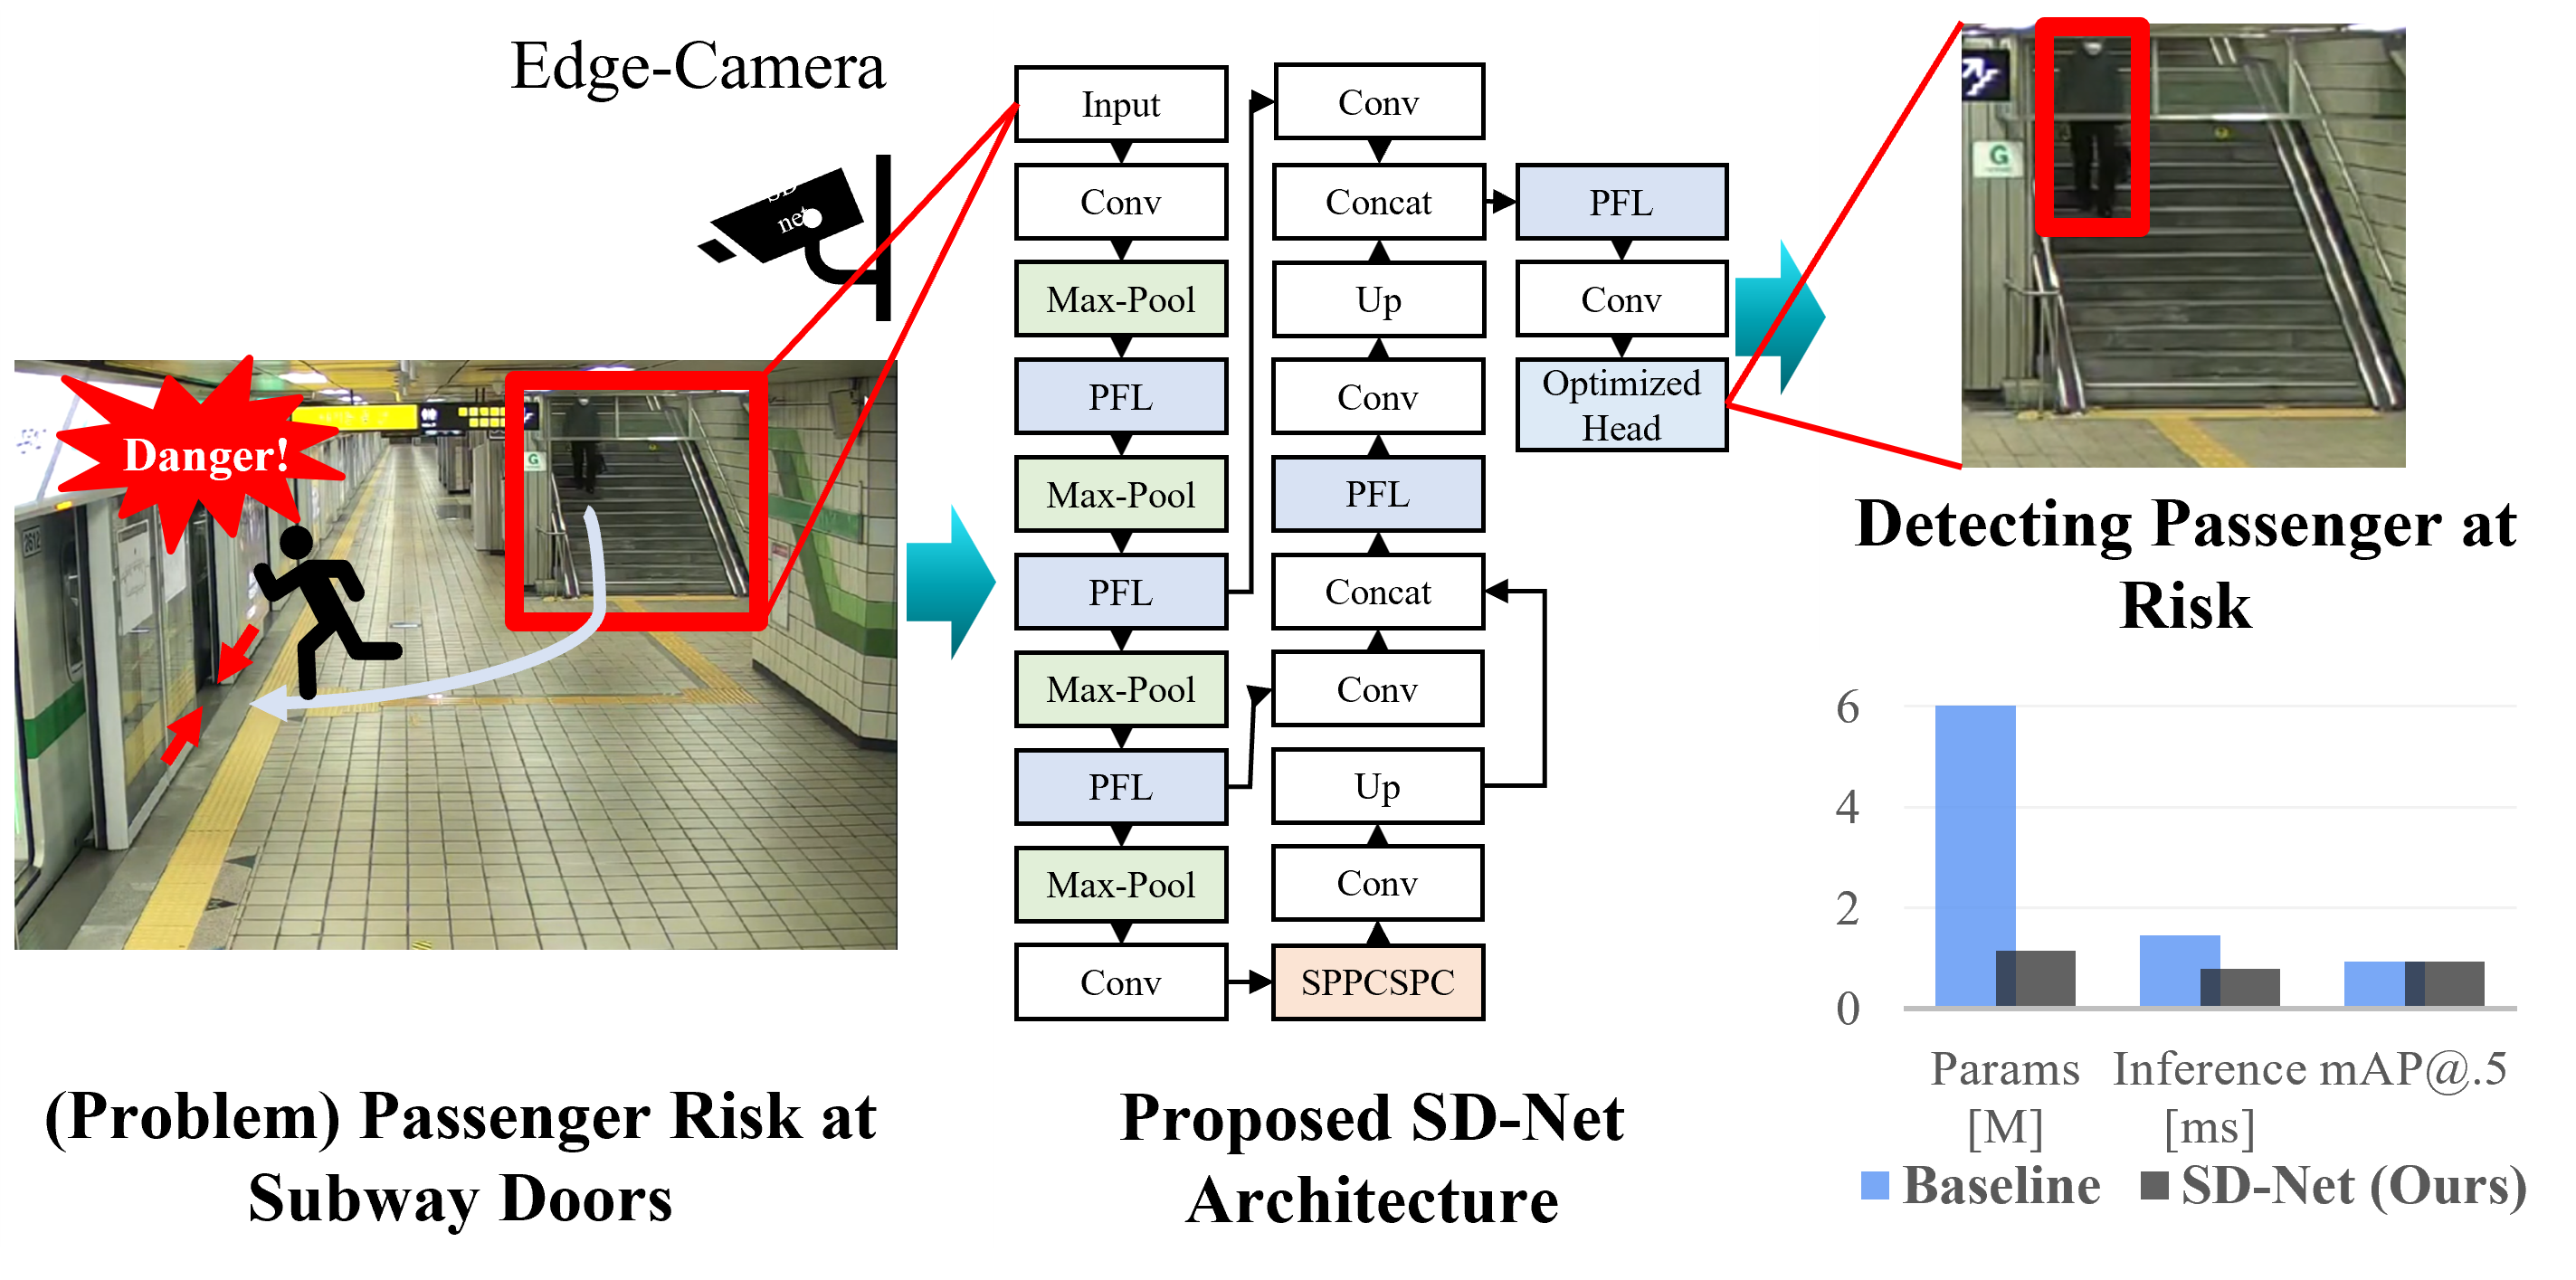
\includegraphics[width=3in]{figures/fig_abstract.png}%
        \end{wrapfigure}%
        \begin{abstract}
            Accidents involving passengers being trapped in subway train doors remain a critical safety issue, despite the presence of conductors’ oversight and platform screen doors. This study proposes Safe Door Network (SD-Net), a lightweight and optimized object detection model designed to accurately detect passenger behavior, particularly stair descent, which precedes most boarding-related door entrapment incidents. 
            Leveraging YOLOv7-tiny as a baseline, we introduce structural modifications to the backbone, neck, and detection heads. These changes include integrating a novel PFL block on backbone and neck and optimization of anchor boxes using Best Possible Recall (BPR) metrics and genetic algorithms. 
            The proposed SD-Net model, trained on a CCTV-based dataset from Seoul Metro, achieves competitive detection accuracy (mAP@0.5 of 93.6\%) while reducing parameter count by over 81.0\% and enhancing inference speed by 45.7\% compared to the baseline YOLOv7-tiny model. These results demonstrate the model's suitability for real-time deployment in resource-constrained edge devices, providing a proactive mechanism to support safety interventions and prevent passenger door accidents in subway systems.
        \end{abstract}
        \begin{IEEEkeywords}
            deep learning, dwell time, edge camera, HAR, passenger trajectory model, train door safety.
        \end{IEEEkeywords}
    \end{minipage}}
}

\maketitle


\section{Introduction}
\label{sec:introduction}
\IEEEPARstart{A}{}tragic accident occurred on May 7, 2025, on São Paulo’s Line 5-Lilás metro line, where a passenger was fatally crushed while attempting to board a train—despite the presence of \acp{PSD} \cite{francisco_lima_neto_passenger_2025}. A similar incident took place on January 22, 2022, at Qi’an Road Station on Shanghai Metro’s Line 15, where an elderly woman was caught by the closing doors and later died from her injuries \cite{Wenting2022Shanghai}. Although such incidents are relatively rare, they highlight persistent vulnerabilities in subway safety systems worldwide. Between 1999 and 2012, for instance, there were 75 injury incidents on London Underground’s Jubilee Line, including cases where passengers' heads and arms were struck by PSD  \cite{Hill2012FOI}. Despite being designed with safety as a primary concern and operated under the strict supervision of train crews and station staff, subway systems still have accidents of passengers' getting caught between train doors \cite{Ahmed2024Guardian, RAIB2024Enfield, RAIB2018Bushey, RAIB2022WoodStreet}. These door-entrapment hazards occur across various subway networks, regardless of whether \acp{PSD} are installed, whether crew members (e.g., train engineers or conductors \cite{swerdlow_underground_1998}) are present, or the level of train automation \cite{RAIB2024Enfield, Kim2024Sillim}.

Passengers typically enter the platform via three main access points: (1) stairs, (2) elevators, and (3) transfer corridors. Among these, the stairway is the most commonly used route. When operating the train doors, the conductor visually checks the platform through \ac{CCTV} \cite{swerdlow_underground_1998}, focusing on these three access routes. In the case of stairs, the conductor determines whether any passengers are descending, whether they intend to board, and estimates their walking speed before deciding to close the doors. However, such visual judgment is inherently limited and prone to human error. Consequently, there is always the possibility that a conductor may fail to notice a passenger approaching via the stairs \cite{RAIB2024Enfield, bayliss2025passenger}. 
This risk highlights the need for an automated visual detection system capable of identifying passenger behavior near these access points, particularly the stairway, in real time.
This risk highlights the need for an automated visual detection system capable of identifying passenger behavior near these three access points, particularly the stairway, in real time.

In this context, our focus is on detecting passengers who are descending the stairs—a key indicator of imminent boarding intent. While traditional \ac{HAR} methods often rely on sequential image data to analyze motion patterns, many human actions, including stair use, can be accurately inferred from a single image frame. Activities such as ascending, descending, or passing by can typically be distinguished based on posture, orientation, and relative position within a frame, even in the absence of temporal context.

Recent advancements in deep learning-based object detection technologies have expanded its adoption across various industrial domains \cite{li2024development}. In the railway field, object detection is being actively explored and increasingly adopted for a variety of safety-critical tasks, such as detecting cracks on rail surfaces \cite{d2024automated}, identifying intrusions in restricted areas \cite{cao2024railway}, assessing rail alignment, and monitoring pantograph (the roof-mounted device that collects electric energy from overhead contact lines \cite{wu2017pantograph}) conditions \cite{li2025branch}. These applications aim to enhance operational safety, reduce maintenance costs, and improve the reliability of railway infrastructure. The integration of object detection models into real-world systems has been accelerated not only by gains in model accuracy and robustness, but also by the availability of large-scale annotated datasets and advances in computing resources. As railway systems move toward greater automation and intelligence, there is a growing need for detection architectures that are efficient, adaptable, and resilient under diverse operational conditions \cite{nold2023will}.

To support the widespread adoption of object detection systems, many researchers and organizations have embraced open-source practices, providing public access to models and their associated pre-trained weights. This openness has simplified deployment across diverse application domains \cite{redmon2016you, jocher2020ultralytics}. A wide range of off-the-shelf models is now available, offering trade-offs in model size, computational complexity, and detection accuracy \cite{wang_yolov7_2022, wang_yolov9_2024, tan2020efficientdet}. Such accessibility has not only lowered the barriers to adoption but also accelerated development cycle, enabling practitioners to select models that align with their operational constraints (e.g., computational resources, real-time performance) and domain-specific requirements. However, despite this widespread adoption for general-purpose tasks, the application of object detection to proactively identify high-risk passenger behaviors for preventing subway door accidents remains largely unexplored. This highlights a critical gap between the available technology and its specific application in enhancing passenger safety at platform access points. 

Various publicly released models are typically evaluated using large-scale benchmark datasets such as PASCAL VOC \cite{everingham_pascal_2010, everingham_pascal_2015}, \ac{MS COCO} \cite{lin_microsoft_2014}, ImageNet \cite{deng2009imagenet}, which facilitate objective comparisons of model performance. In particular, the \ac{MS COCO} dataset has become a widely adopted standard, particularly with the emergence of \acp{ViT}, some of which have achieved over 60\% \ac{mAP} at \ac{IoU} threshold 0.5 (mAP@0.5) \cite{zhang2022dino}. Fig.~\ref{fig:01a_stacked} presents the log-scale histogram of object width, height, and area distributions within the \ac{MS COCO} dataset. The $x$-axis represents the object dimensions (width, height, and area) normalized by the image size, while the $y$-axis indicates the frequency. As shown in the figure, although small objects dominate, object sizes are distributed across the entire range from very small to very large. In contrast, Fig. 1b presents the distribution in the passenger dataset used in this study, where object sizes are more concentrated, with most object widths and heights concentrated around 0.2 and 0.55, respectively. Note that there are almost no objects exceeding 0.6 in width or 0.7 in height. 

\begin{figure}[ht]
    \centering
    
    \begin{subfigure}[b]{0.45\textwidth} % Adjust width as needed
        \centering
        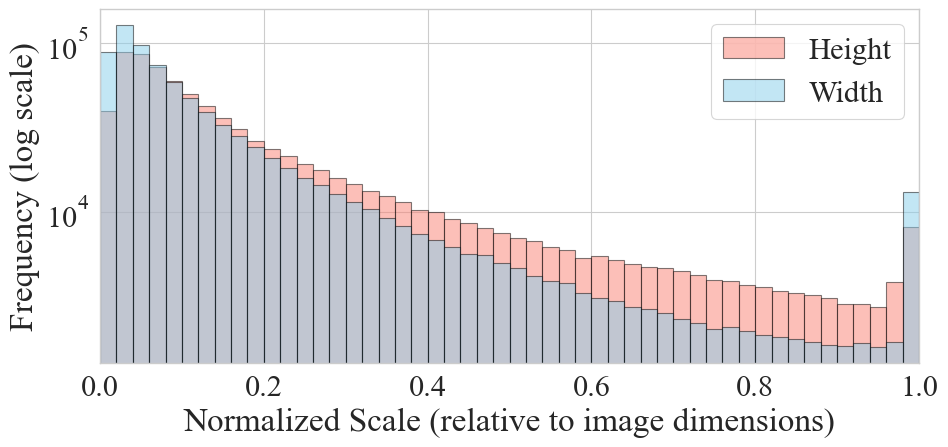
\includegraphics[width=\textwidth]{figures/histo_coco.png}
        \caption{Normalized width, height, and area in the MS COCO dataset}
        \label{fig:01a_stacked}
    \end{subfigure}
    
    \vspace{1em} % Adds a little vertical space
    
    \begin{subfigure}[b]{0.45\textwidth} % Adjust width as needed
        \centering
        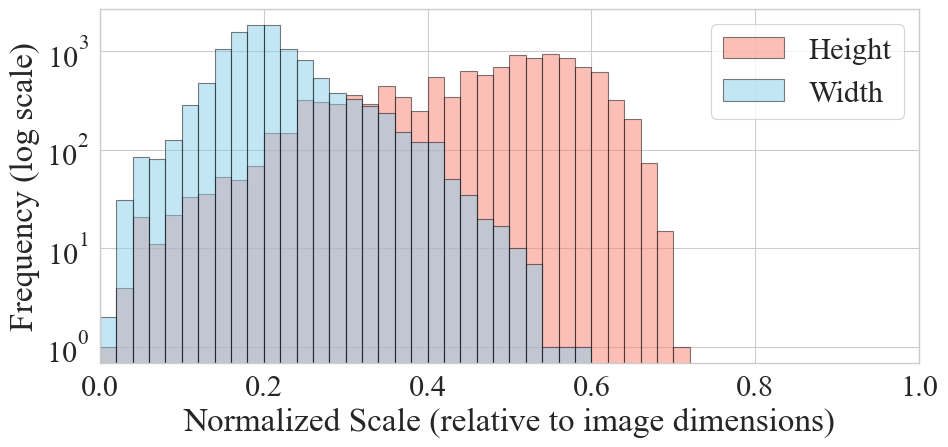
\includegraphics[width=\textwidth]{figures/histo_passenger.png}
        \caption{Normalized width, height, and area in the passenger dataset}
        \label{fig:01b_stacked}
    \end{subfigure}
    
    \caption{(a) Log-scale histograms of normalized width, height, and area distributions in the \ac{MS COCO} dataset  \cite{lin_microsoft_2014} and (b) the passenger dataset used in this study. Object dimensions are normalized with respect to each image size. \ac{MS COCO} exhibits a broad range of object sizes, whereas the passenger dataset shows a more concentrated size distribution.}
    \label{fig:data_hist_comparison}
\end{figure}

% This contrast in distributions, shown in Fig. \ref{fig:data_hist_comparison}, reveals a key insight: general-purpose models are designed for the high variance of datasets like MS COCO. To achieve this, they dedicate significant computational resources and parameters—for example, by using a complex backbone, multiple detection heads, and a multi-scale anchor box strategy—all designed to achieve scale-invariance.

This contrast in distributions, shown in Fig.~\ref{fig:data_hist_comparison}, reveals a key insight: general-purpose models are designed for the high variance of datasets like \ac{MS COCO}.
To formally quantify this observed difference in complexity, we calculated the Shannon entropy ($H(X)$) of the normalized object dimension distributions \cite{bromiley2004shannon}. 
This metric measures the uncertainty or diversity of a distribution. 
For a probability distribution $P$ discretized into $n$ bins, where $P(x_i)$ is the probability of an object falling into bin $i$, the entropy is calculated as:

\begin{equation}
\label{eq:entropy}H(X) = - \sum_{i=1}^{n} P(x_i) \log_2(P(x_i))
\end{equation}

Applying this (using 50 common bins) to the distributions from Fig.~\ref{fig:data_hist_comparison}, our passenger dataset showed significantly lower entropy for relative width (3.62 bits) and height (4.43 bits) compared to \ac{MS COCO} (4.47 and 4.85 bits, respectively). This low entropy score provides quantitative proof of our dataset's predictability and supports the hypothesis that a simplified architecture is sufficient.





% A formal statistical analysis, detailed in Section~\ref{sec:entropy_analysis}, confirms that our passenger dataset's object size distribution is significantly more concentrated and predictable.

To accommodate the high variance found in \ac{MS COCO} dataset, general-purpose models dedicate significant computational resources and parameters, for example, by using a complex backbone, multiple detection heads, and a multi-scale anchor box strategy.
These structural elements are designed not only to achieve scale-invariance but also to enhance localization precision and resolve overlapping objects.
While this complexity is necessary for high accuracy on those general benchmarks, it arguably represents computational inefficiency when applied to a specialized task like our passenger dataset, where object sizes are highly consistent. 

This insight forms the motivation for our work: we hypothesize that a lightweight, specialized architecture—which relies on a simplified backbone and fewer detection heads—can be designed to achieve competitive accuracy while being far more efficient, making it suitable for real-time deployment on resource-constrained edge devices.

This relatively narrow distribution of object sizes in the passenger dataset may allow for more efficient model architecture, as less emphasis is needed on scale-invariant design components.


Building on this insight, we propose an object detection–based approach for behavior recognition, which diverges from conventional sequence-based \ac{HAR} strategies. Among state-of-the-art object detectors, \ac{YOLO} is widely adopted for its strong balance between accuracy and inference speed. 
% In Chapter 2, our empirical evaluations demonstrated that YOLOv7-tiny already achieved exceptional real-time potential (630 FPS) while maintaining a highly competitive mAP@0.5 of 97.58\%. Furthermore, unlike other YOLO iterations that rely heavily on dense, intertwined cross-stage partial networks, YOLOv7-tiny utilizes the Extended Efficient Layer Aggregation Network (E-ELAN). This modular architecture is uniquely suited for systematic pruning; it allows for the structural simplification of convolutional blocks without severely disrupting the gradient flow.
In this study, we introduce the \ac{SD-Net}, an optimized architecture based on YOLOv7-tiny \cite{wang_yolov7_2022}, to detect specific passenger behaviors, with the aim of preventing door entrapment incidents on subway platforms.

We conduct experiments, following the optimization process shown in Fig. 2, adjusting the backbone structure, head design, and anchor box configuration to develop a lightweight, yet effective model tailored to our custom dataset. 
The result is a task-specific object detection framework optimized for real-time deployment in safety-critical subway environments.



The main contributions of this study are as follows:
\begin{itemize}
    \item We introduce \ac{SD-Net}, a novel, lightweight architecture specifically designed to make the proactive prevention of subway door accidents computationally feasible for real-time, resource-constrained edge devices.
    
    \item We present a data-driven optimization strategy that simplifies the detection head and anchor boxes based on our dataset's specific object characteristics, and introduce the highly efficient \ac{PFL} block as a new architectural component.
    
    \item We validate that \ac{SD-Net} achieves a drastically reduced model size and significantly faster inference speed compared to the YOLOv7-tiny baseline, all while maintaining competitive detection accuracy.
\end{itemize}

\begin{figure}[!t]
    \centerline{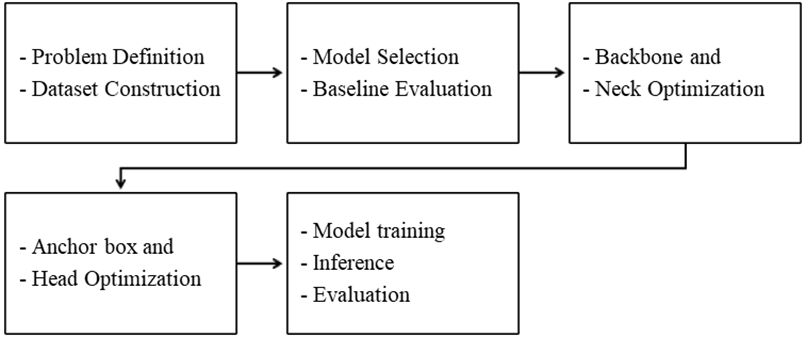
\includegraphics[width=\columnwidth]{figures/fig_02.png}}
    \caption{The proposed passenger behavior detection and model optimization process.}
    \label{fig:whole_process}
\end{figure}


\section{Related Works}
The objective of this study is to design an optimal object detector that enables a proactive system for preventing subway door entrapment accidents. This is achieved by focusing on the real-time detection of passengers descending a staircase when a train is present at the station. In this section, we provide a comprehensive review of the advancements in object detection research, encompassing the evolution of backbone architectures, detection heads, and anchor box strategies. Furthermore, we examine prior studies that have addressed the prevention of accidents involving subway doors.  

\subsection{Development of Backbone of Object Detector}
Early deep‐learning object detectors combined \acp{CNN} with fully connected layers \cite{girshick2014rich, redmon2016you}. These evolved into \acp{FCN}, which dramatically improved spatial feature extraction. Key innovations such as ResNet’s skip connections \cite{he2016deep}, VoVNet’s One-Shot Aggregation \cite{lee2019energy}, and DenseNet’s dense connectivity \cite{huang2017densely} enabled much deeper networks to train effectively. 

Concurrently, there has been a push toward computationally efficient and lightweight backbones. Models like MobileNet \cite{howard2017mobilenets} and ShuffleNet \cite{zhang2018shufflenet} leverage depthwise‐separable convolutions and channel shuffling to minimize operations while retaining accuracy. Such designs are indispensable for real-time detection on edge and mobile devices. 

More recent work has explored hybridizing lightweight modules with proven high-capacity structures. YOLOv7 \cite{wang_yolov7_2022}, for example, integrates concepts from DenseNet within its \ac{ELAN} backbone. In this study, we further tailor YOLOv7’s backbone—introducing \ac{PFL} blocks and replacing early convolutions with max-pooling—to reduce parameters and \ac{FLOPS} while maintaining detection performance on our passenger dataset.


\subsection{Development of Head of Object Detector}
Detection heads have similarly progressed through two paradigms: two-stage and one-stage architectures.

Two-stage detectors, such as those in the R-CNN \cite{girshick2014rich} family (e.g., Faster R-CNN \cite{ren2016faster}), first generate candidate object regions using an \ac{RPN}. These proposals are then refined through subsequent classification and bounding box regression stages. While such models achieve high detection accuracy, their multi-phase structure introduces considerable computational cost, making them less suitable for real-time applications. To address these limitations, one-stage detectors emerged. Models like YOLO \cite{redmon2016you} and SSD \cite{liu2016ssd} predict object classes and bounding boxes directly from feature maps in a single forward pass, offering a substantial improvement in speed. More recent models such as YOLOv9 \cite{wang2024yolov9}, CenterNet \cite{duan2019centernet} and FCOS \cite{tian2019fcos} have further innovated by eliminating anchor boxes and instead directly regressing object centers or box boundaries.  


The YOLO family, in particular, has undergone continuous refinement to improve both efficiency and detection accuracy. In this study, we began with the YOLOv7-tiny architecture and observed that reducing the backbone’s complexity only minimally impacted \ac{mAP}. Simplifying the backbone increased the relative computational burden of the remaining detection heads, clearly identifying them as the new optimization bottleneck. Given that our passenger dataset consists of objects with consistent aspect ratios and visual features, a heavily parameterized detection head was likely unnecessary. We therefore conducted experiments to simplify the head architecture by reducing the number of detection heads. This approach allowed us to enhance inference speed and lower computational load while maintaining detection performance, aligning with the study's goal of real-time deployment in safety-critical subway environments.

The YOLO family, in particular, has undergone continuous refinement to improve both efficiency and detection accuracy. In this study, we began with the YOLOv7-tiny architecture and observed that reducing the backbone’s complexity only minimally impacted \ac{mAP}. As a result, the relative computational burden of the head increased. 
Given that our passenger dataset consists of objects with consistent aspect ratios and visual features, a heavily parameterized detection head was likely unnecessary. We therefore conducted experiments to simplify the head architecture by reducing the number of detection heads and optimizing channel distribution. This approach allowed us to enhance inference speed and lower computational load while maintaining detection performance, aligning with the study's goal of real-time deployment in safety-critical subway environments. 

\subsection{Anchor Box Optimization}
The anchor box is one of the critical factors that determine the bounding box prediction performance in object detection models. It serves as a predefined bounding box that represents the distribution of the training dataset. In YOLOv2 \cite{redmon2017yolo9000}, \ac{IoU}-based $k$-means clustering was adopted to partition the distribution of object shapes (width and height) in the training dataset into $k$ clusters.
They found the anchor box that minimizes the distance function $d(\text{box}, \text{anchor}) = 1 - \text{IoU}(\text{box}, \text{anchor})$, and the centroids of each cluster were used as anchor boxes. By calculating the average \ac{IoU} between the bounding box of the object and anchor boxes for different values of $k$, it was demonstrated that the average \ac{IoU} increases as the number of anchor boxes increases. Consequently, an optimal trade-off point for $k$ was selected manually for recall versus model complexity \cite{redmon2017yolo9000}.

In YOLOv5 \cite{jocher2020ultralytics}, the \ac{BPR} method is employed to evaluate the quality of anchor boxes. They used \ac{GA} to evolve the anchor boxes by maximizing the fitness function, \ac{BPR}. While YOLOv2 measures anchor box quality using average \ac{IoU}, YOLOv5's \ac{BPR} instead assesses the number of objects whose width and height ratios relative to the anchor box exceed a predefined threshold $\tau$. For each object, $k$ anchor boxes are assigned, and the best-matching anchor box among them is selected. \ac{BPR} thus quantifies the proportion of objects that are sufficiently covered by at least one anchor box—that is, those for which the minimum of the width and height ratios relative to the anchor box exceeds a predefined threshold $\tau$—thereby providing a direct indicator of the anchor box configuration’s effectiveness. This is why \ac{BPR} can be interpreted as a form of recall, as it represents the number of objects for which the minimum of the width and height ratios between object and anchor box exceeds the threshold. However, it does not correspond to the recall of object detection precision, since the threshold is manually set and does not inherently reflect the model’s detection capability.

\ac{BPR} serves as an evaluation metric that assesses the effectiveness of anchor boxes based on object size (width and height) ratios. It operates by calculating the ratio between each anchor box and the object dimensions in the dataset, selecting the anchor box with the highest matching score. While YOLOv2's $k$-means clustering approach determines anchor boxes by finding the centroid of object dimensions, \ac{BPR} directly compares width and height ratios without relying on \ac{IoU}, providing a more informative evaluation of anchor box quality. If the target objects vary significantly in size, increasing the number of anchor boxes can improve coverage across diverse object scales. Conversely, if the object sizes are relatively uniform, fewer anchor boxes can still achieve a high \ac{BPR} value. This enables more precise adaptation to object size variations. In this study, various anchor box configurations were explored based on \ac{BPR} evaluations, and the backbone and head structures were optimized to develop a model best suited to the passenger dataset. This approach enabled an analysis of how the number of anchor boxes and detection heads impacts detection performance, ultimately leading to the design of a dataset-optimized detection model.


\subsection{Preventing Passenger Door Accidents}
To prevent passengers from becoming trapped in subway doors, most systems rely on a combination of sensor technologies. These range from contact-based safety edges and motor-current or pressure sensors that detect obstructions by force \cite{yao2024failure, bayliss2025passenger, shiao2024wavelet}, to non-contact methods such as optical or laser scanners that monitor the gap between the train and platform screen doors \cite{BEA2025FlatscanS, SICK2025LidarSensors}. Another camera-based approach places LED lights at the bottom of the platform and monitors them for obstructions, demonstrating potential for identifying entrapment events at the platform edge \cite{lu2025urban, heng2025research}. However, all these approaches are inherently reactive, as they respond only when the risk is already imminent.

To address this limitation, our method focuses on identifying risky passenger actions—such as rushing toward train doors—before the passenger reaches the immediate boarding zone. By detecting these behaviors early, the system enables proactive intervention to help prevent accidents before they escalate.

Research has also been conducted on passenger movement patterns and door selection behavior in subway stations \cite{jo_trajectory_2021}. Previous studies have revealed that passengers tend to choose doors along the shortest route when using stairways. By leveraging this insight, it became possible to predict which door passengers descending the stairs would use as the train arrives at the platform. Furthermore, by detecting passengers as they descend the stairs, it was possible to estimate the optimal moment to close the train doors.



\section{Methodology}
The objective of this study is to design an optimized object detection model capable of rapidly and accurately detecting passengers descending the stairs on a subway platform. To achieve this, we use the YOLOv7-tiny model as a baseline and perform systematic optimization of its backbone architecture, head configuration, and the number of anchor boxes, tailored to the characteristics of our custom passenger dataset. This section outlines the methods employed to identify the optimal number of parameters, \ac{FLOPS}, and inference speed suited for the passenger detection task.

\subsection{Backbone Optimization}
In this study, we analyze and modify the \ac{ELAN} structure used in the backbone of YOLOv7-tiny, which is responsible for feature extraction. The architecture of YOLOv7-tiny is shown in Fig. \ref{fig:yolov7_tiny_architecture}. The \ac{ELAN} module in YOLOv7-tiny includes pairs of convolutional layers with identical kernel sizes. For instance, the first \ac{ELAN} block consists of two (32, $1\times1$, stride=1) filters and two (32, $3\times3$, stride=1) filters. The feature maps produced by these four convolution blocks are concatenated and passed through an additional convolutional block.

\begin{figure}[tb]
    \centerline{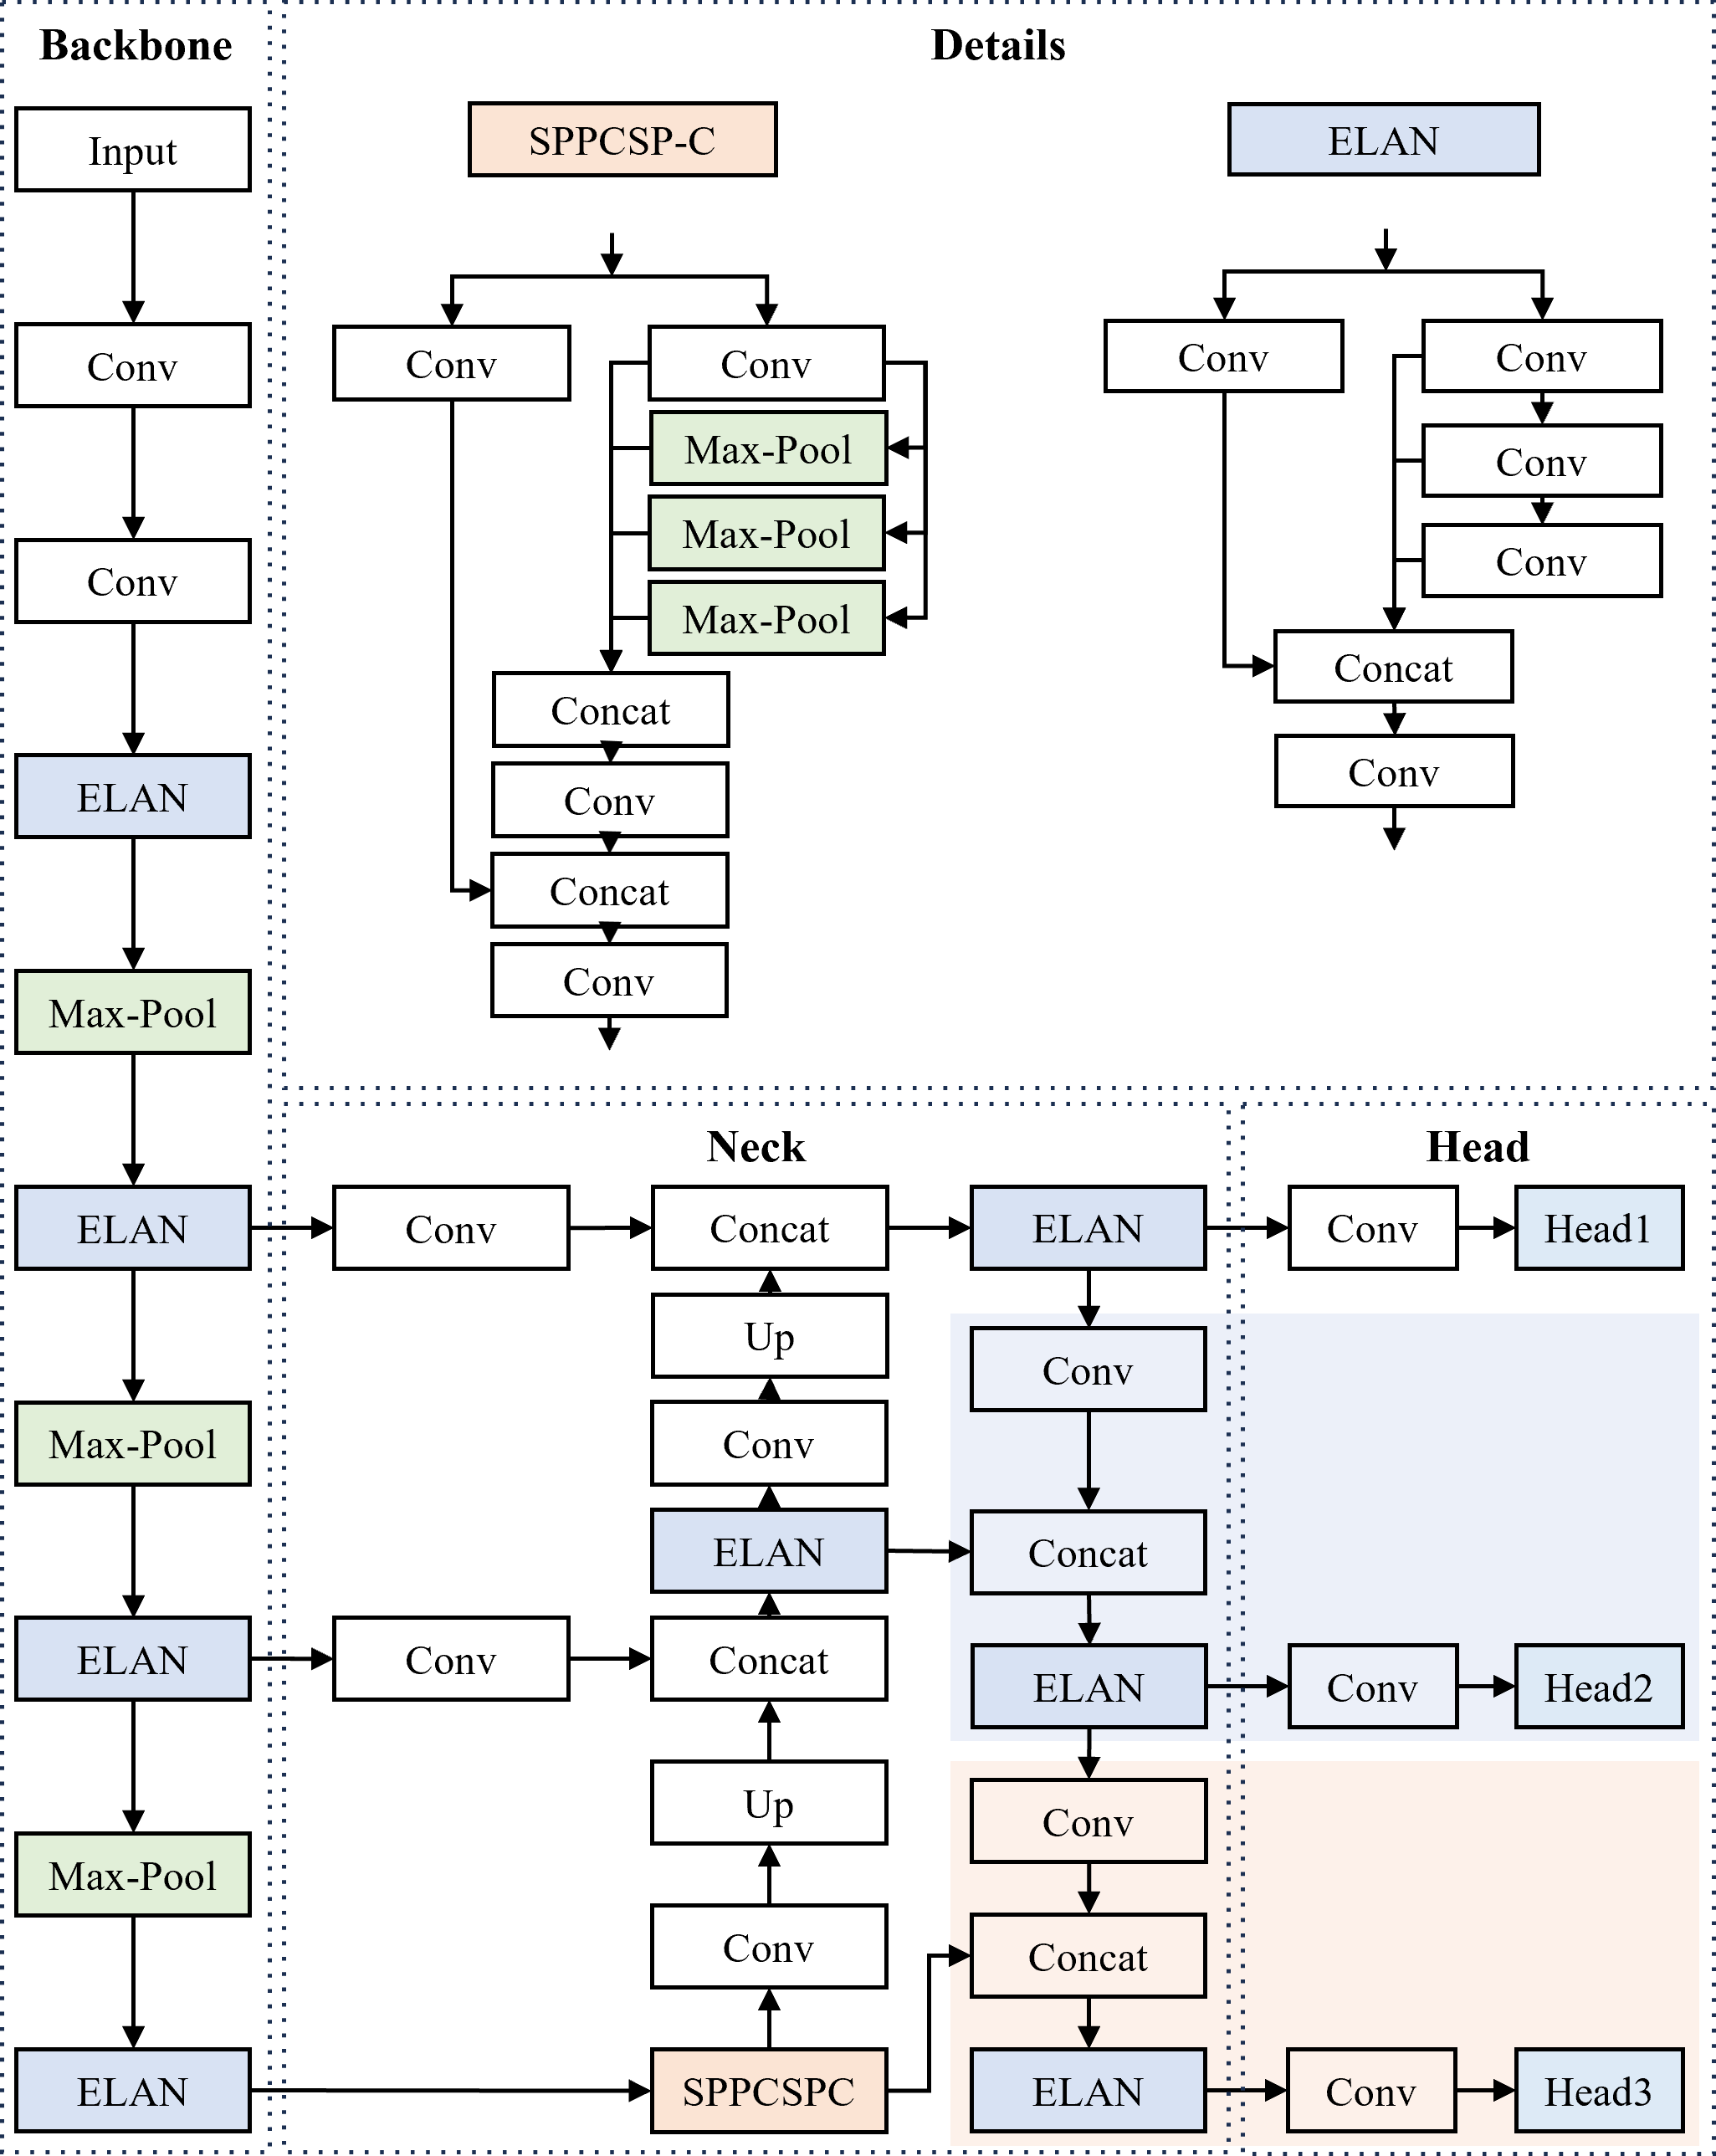
\includegraphics[width=\columnwidth]{figures/fig_03.png}}
    \caption{Network architecture of YOLOv7-tiny. The model includes an \ac{ELAN} block and three detection heads, with a total of 6,020,400 trainable parameters with 263 layers.}
    \label{fig:yolov7_tiny_architecture}
\end{figure}

To reduce the computational load, we systematically removed one duplicated convolutional layer at a time from the initial YOLOv7-tiny’s \ac{ELAN} structure and experimented with lighter configurations. As illustrated in Fig.~\ref{fig:SD_Net_architecture}, we ultimately replaced the \ac{ELAN} block with a \ac{PFL} structure, which preserves detection performance while reducing computational complexity. The \ac{PFL} block splits the input tensor into two parallel paths: one with a (32, $1\times1$, stride=1) convolution and the other with a (32, $3\times3$, stride=1) convolution. The outputs from these paths are then concatenated and passed through a subsequent convolutional block, forming an efficient parallel structure.

\begin{figure}[!t]
    \centerline{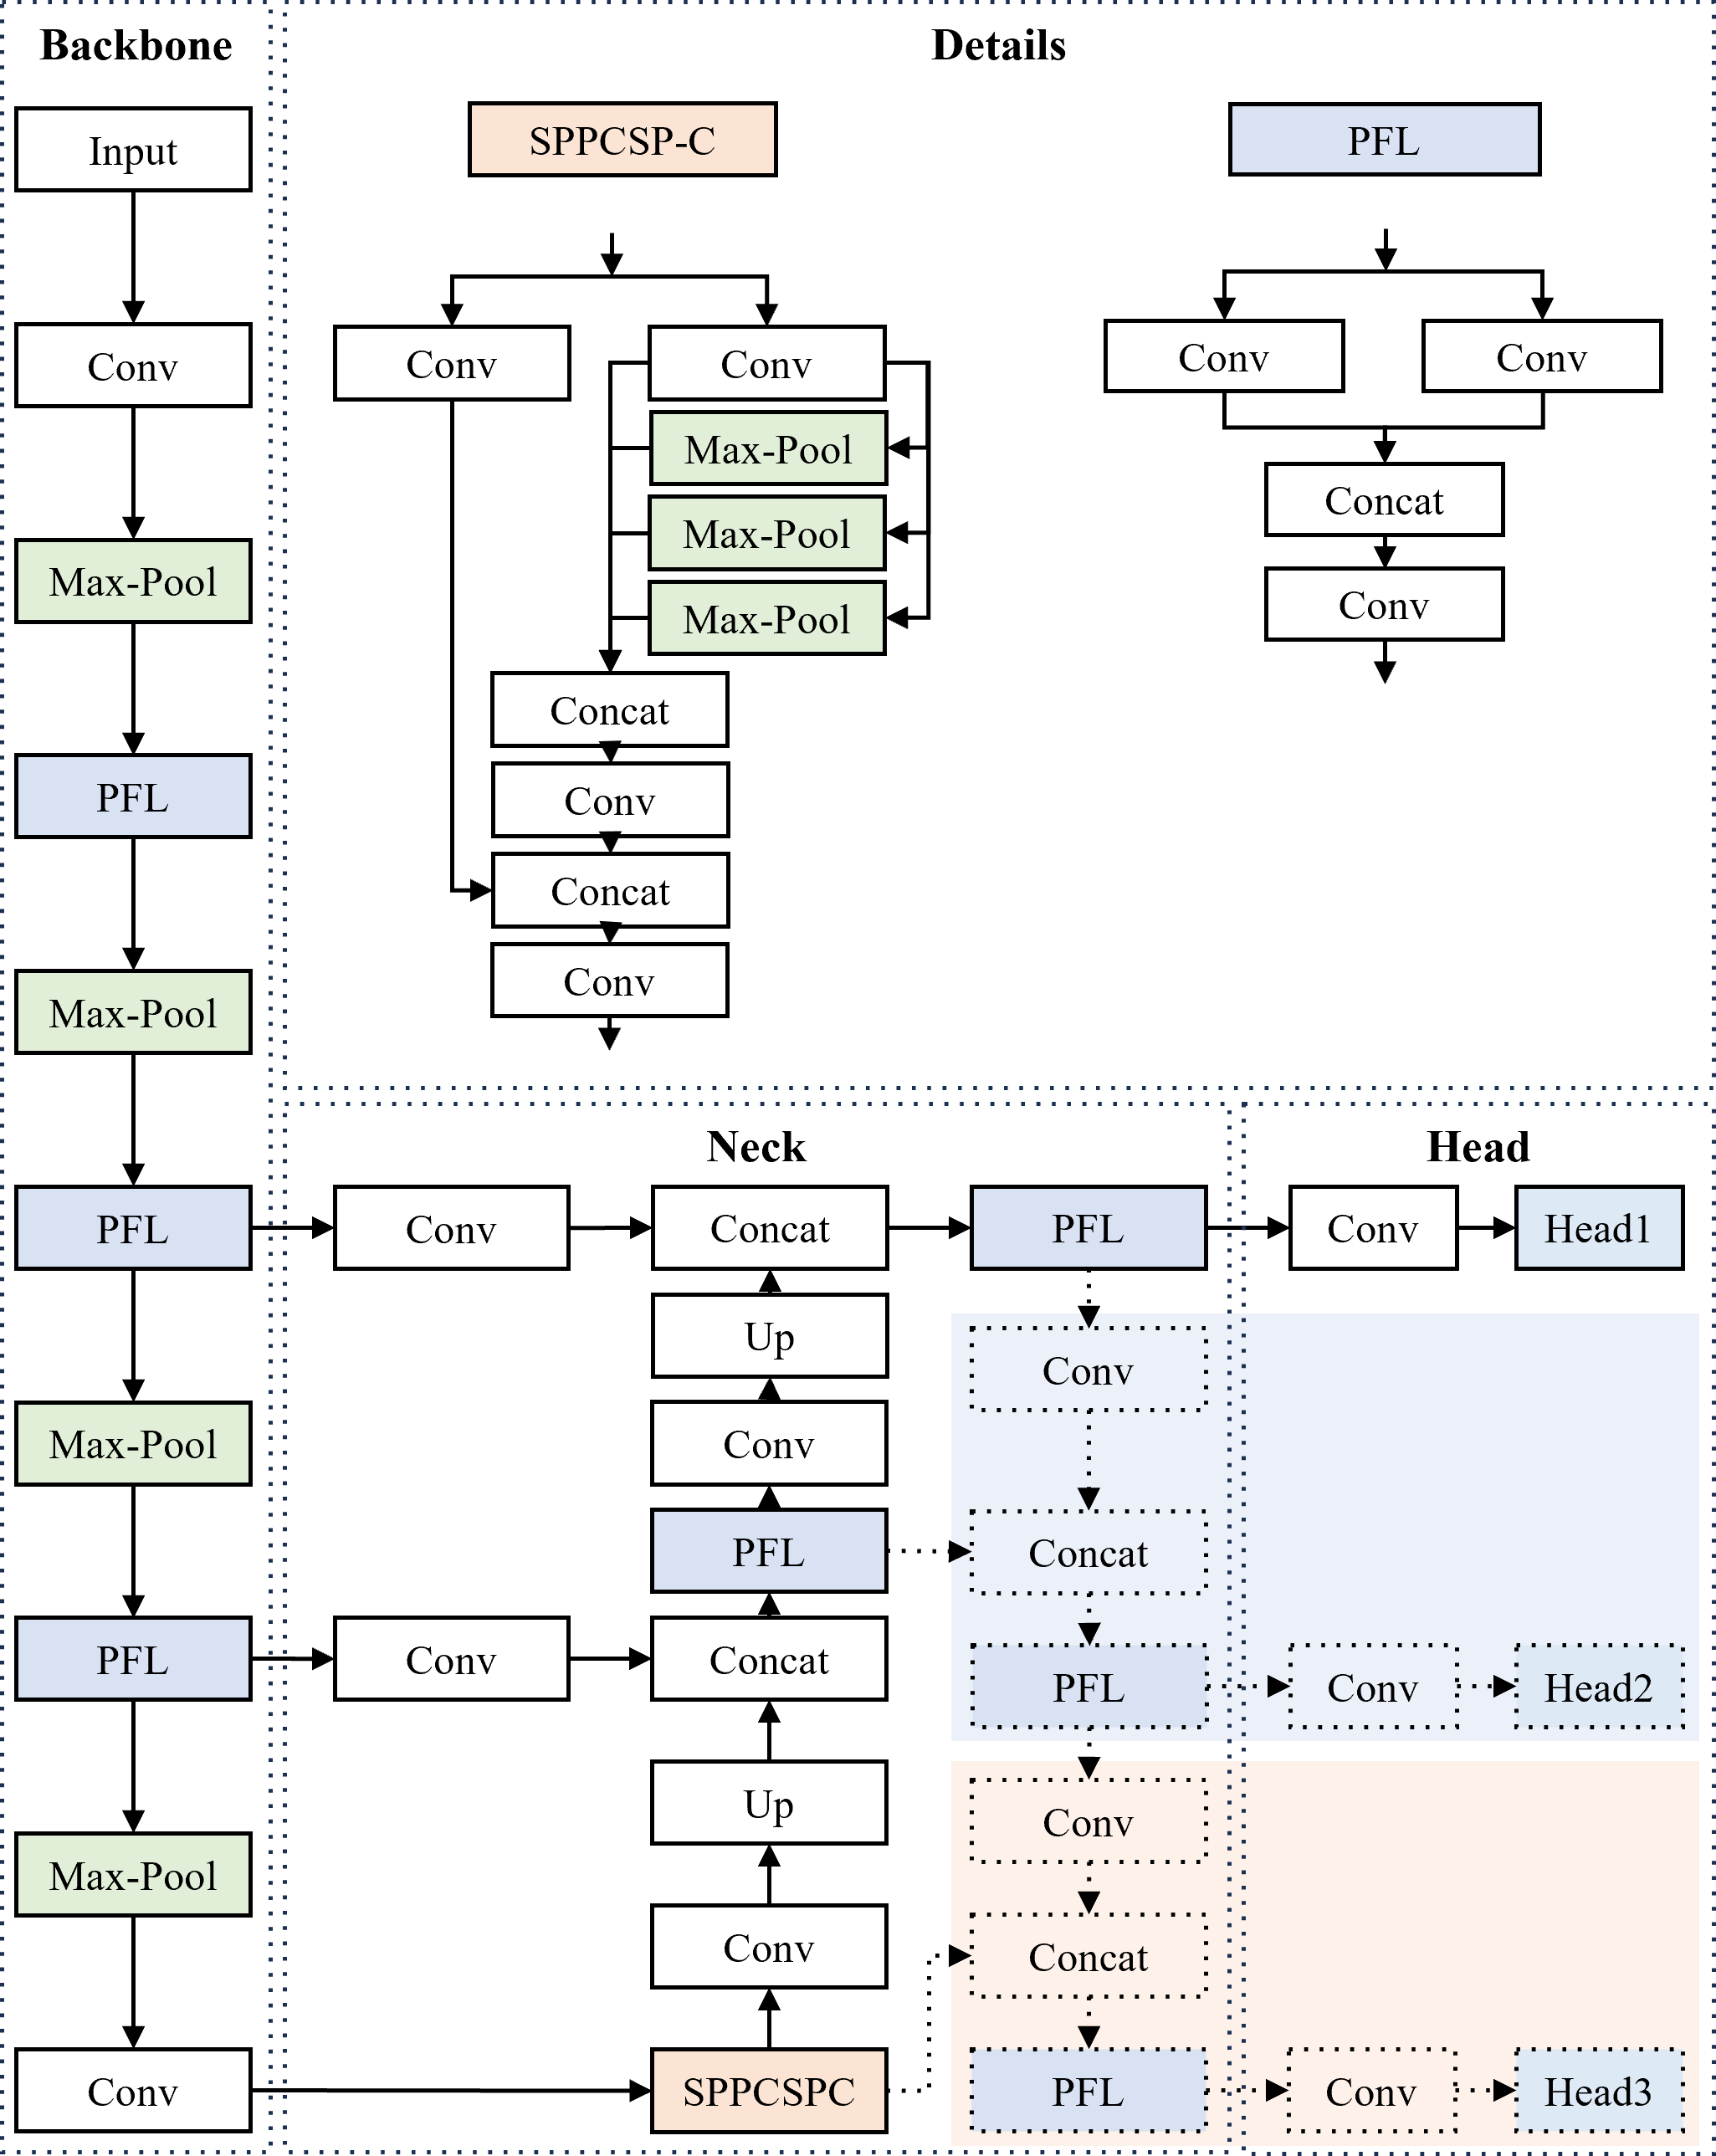
\includegraphics[width=\columnwidth]{figures/fig_04.png}}
    \caption{Proposed network architecture. Compared with yolov7-tiny architecture in Fig. \ref{fig:yolov7_tiny_architecture}, the third layer (Conv) in Fig. \ref{fig:yolov7_tiny_architecture} is replaced with Max-pool layer and the last \ac{ELAN} block in the backbone is replaced with Convolution block. The \ac{ELAN} block in YOLOv7-tiny is replaced with the \ac{PFL} block, and two detection heads (shaded as blue and orange color box) are removed, reducing the number of trainable parameters to 1,148,960 with 138 layers.}
    \label{fig:SD_Net_architecture}
\end{figure}

Additionally, because the sizes of the passengers in our dataset are relatively consistent, we hypothesized that reducing the spatial resolution of feature maps early in the network would not significantly degrade detection performance. Based on this assumption, we introduced a max-pooling layer at the beginning of the model. This approach reduces the spatial dimensions of the feature maps, thereby decreasing the overall computational cost. Moreover, it effectively enlarges the receptive field of subsequent convolutional filters, allowing the model to capture broader contextual information while reducing the number of parameters.


% \subsection{Head and Anchor Box Optimization}
% The baseline YOLOv7-tiny model employs a total of nine anchor boxes, distributed across three detection heads, with each head responsible for detecting objects of small, medium, and large sizes, respectively. However, the dataset used in this study involves passengers captured at fixed distances from a stationary \ac{CCTV} or an edge camera. As a result, the variation in object (passenger) size is minimal. 

% This characteristic is illustrated in Fig. \ref{fig:05_kmeans_distribution}. Fig. \ref{fig:05a} shows the results of applying $k$-means clustering (with $k=6$) to the bounding box dimensions of the training dataset. Each cluster centroid, marked with a red “$\times$”, represents candidate anchor box. It uses pixel values on both the $x$- and $y$-axes ranging from 0 to 320, so the position of each point from the origin directly corresponds to the width and height of an individual object (bounding box) in the dataset.

% The right plot (Fig. \ref{fig:05b}) shows the histograms of object widths and heights in pixel domain, confirming the concentration as we discussed in the \ref{fig:01b_stacked}: most objects are clustered around a width of 70 pixels and a height of 175 pixels. This uniformity implies that a complex, multi-scale head design is likely unnecessary.


\subsection{Head and Anchor Box Optimization}
The baseline YOLOv7-tiny model employs a total of nine anchor boxes, distributed across three detection heads, with each head responsible for detecting objects of small, medium, and large sizes, respectively. However, the dataset used in this study involves 
passengers captured at fixed distances from a stationary \ac{CCTV} or an edge camera. As a result, the variation in object (passenger) size is minimal. 

This characteristic is illustrated in Fig. \ref{fig:05_kmeans_distribution}. Fig. \ref{fig:05a} shows the results of applying $k$-means clustering (with $k=6$) to the bounding box dimensions of the training dataset. Each cluster centroid, marked with a red “$\times$”, represents a candidate anchor box. It uses pixel values on both the $x$- and $y$-axes ranging from 0 to 320, so the position of each point directly corresponds to the width and height of an individual object (bounding box) in the dataset.

The right plot (Fig. \ref{fig:05b}) shows the histograms of object widths and heights in the pixel domain on a linear scale, confirming the concentration previously shown in Fig. \ref{fig:01b_stacked}: most objects are clustered around a width of 70 pixels and a height 
of 175 pixels. This uniformity implies that a complex, multi-scale head design is likely unnecessary.

% \label{sec:entropy_analysis}
% As shown earlier in Fig.~\ref{fig:data_hist_comparison}, the MS COCO dataset includes a wide range of object sizes spanning the entire image scale, necessitating diverse anchor boxes.
% In contrast, the passenger dataset exhibits size homogeneity, suggesting that a smaller and more focused set of anchor boxes may be sufficient.
% To formally quantify this observed difference in complexity, we calculated the Shannon entropy ($H(X)$) of the normalized object dimension distributions \cite{bromiley2004shannon}. This measures the uncertainty or diversity of a distribution. For a probability distribution $P$ discretized into $n$ bins, where $P(x_i)$ is the probability of an object falling into bin $i$, the entropy is calculated as \cite{bromiley2004shannon}:

% \begin{equation}
%     \label{eq:entropy}
%     H(X) = - \sum_{i=1}^{n} P(x_i) \log_2(P(x_i))
% \end{equation}

% Applying this (using 50 common bins) to the distributions from Fig.~\ref{fig:data_hist_comparison}, our passenger dataset showed significantly lower entropy for relative width (3.62 bits) and height (4.43 bits) compared to MS COCO (4.47 and 4.85 bits, respectively). This low entropy score provides quantitative proof of our dataset's predictability and supports the hypothesis that a simplified head architecture is sufficient.

\begin{figure}[!t]
    \centering % Center the whole figure
    % --- Sub-figure (a) ---
    \begin{subfigure}[b]{0.48\columnwidth}
        \centering
        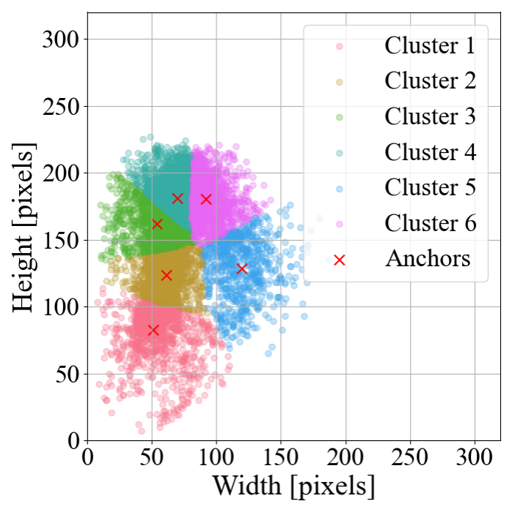
\includegraphics[width=\textwidth]{figures/fig_05a.png}
        \caption{Result of $k$-means clustering ($k=6$)} % Your caption for fig_05a
        \label{fig:05a}
    \end{subfigure}
    \hfill % Adds horizontal space between the two images
    \begin{subfigure}[b]{0.48\columnwidth}
        \centering
        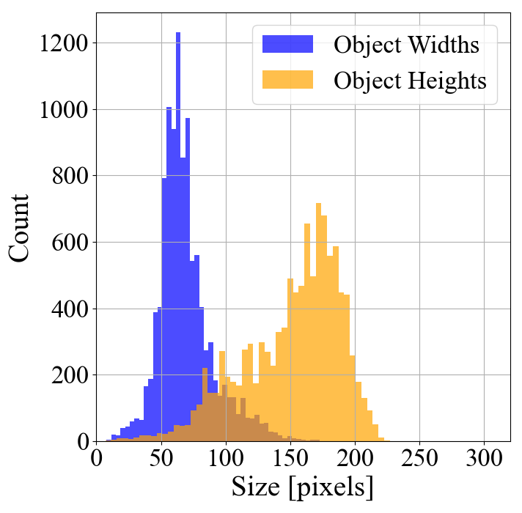
\includegraphics[width=\textwidth]{figures/fig_05b.png}
        \caption{Histogram of object width and height} % Your caption for fig_05b
        \label{fig:05b}
    \end{subfigure}
    \caption{(a) The result of $k$-means clustering of anchor boxes with $k=6$ and (b) the distribution of width and height of the training dataset. Most of the width and the height of object (passenger) is concentrated around 70 and 175 pixels respectively. \textbf{ This will be changed to k=8 !!!}}
    \label{fig:05_kmeans_distribution}
\end{figure}


\begin{figure}[!t]
    \centering
    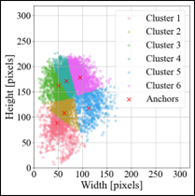
\includegraphics[width=0.5\columnwidth]{figures/fig_07.png}
    \caption{$k$-means clustering of Anchor boxes after applying generic algorithm. Compared to Fig. 5a, the anchor boxes are slightly changed. The BPR for Fig. 5a is 0.9140 at threshold of 0.75, and the BPR for Fig. 7 is 0.9320 at threshold of 0.75. By using generic algorithm, the BPR is increased by about 1.8\%. \textbf{This will be updated to k=8 case too with anchor box plots !!!}}
    \label{fig:k-mean clusturing}
\end{figure}


Based on this insight, we conducted experiments to reduce the number of detection heads under the assumption that fewer scales would suffice for effective detection. 
We evaluated the YOLOv7-tiny baseline and our proposed model with progressively fewer heads—three, two, and one—while comparing their detection performance. The architecture with a single detection head is shown in Fig. \ref{fig:SD_Net_architecture}, where the layers marked with blue and orange boxes are excluded. The two-head version includes only the blue-box layers, while the three-head version includes both.
For each head configuration, we tested various combinations of anchor box counts to determine optimal performance. In object detection models, anchor boxes are predefined bounding boxes that play a crucial role in matching predictions with ground truth objects. Proper selection of anchor box dimensions significantly affects detection accuracy \cite{redmon2017yolo9000}.

YOLOv2 introduced a method for selecting anchor boxes based on $k$-means clustering, which finds an optimal number of anchor boxes by evaluating the trade-off between average IoU and the number of clusters. Later, YOLOv5 \cite{jocher2020ultralytics} introduced the \ac{BPR} metric along with a genetic algorithm to optimize anchor boxes more effectively. Unlike earlier methods, \ac{BPR} does not rely on \ac{IoU}. Instead, it compares the width and height of each object to those of $k$ anchor boxes, selects the best match for each object, and evolves anchor box configurations using a genetic algorithm.

\ac{BPR} measures how well the predefined anchors match the object shapes in the (training) dataset. We first define the object bounding boxes as width-height pairs $(w_i, h_i) \in \mathbb{R}^2$ for $i=1, \dots, N$, where $N$ is the total number of objects in the training dataset. Similarly, let the $k$ predefined anchor boxes be defined as $(w_j, h_j) \in \mathbb{R}^2$ for $j=1, \dots, k$. The matching ratio matrix $R \in \mathbb{R}^{N \times k}$ is then computed as shown in Equation (\ref{eq:bpr_ratio}).

\begin{equation}
R_{i,j} = \min\left(\frac{w_i}{w_j}, \frac{w_j}{w_i}, \frac{h_i}{h_j}, \frac{h_j}{h_i}\right)
\label{eq:bpr_ratio}
\end{equation}

Each element $R_{i,j}$ represents the smallest of the width or height ratios between the $i$-th object and the $j$-th anchor box. This ratio quantifies how well the shape of each anchor box aligns with the shape of each object by choosing the worst mismatch ratio value. If we use six anchor boxes ($k=6$), for each object $i$, we now have six corresponding values $R_{i,j}$. We then select the best-matching anchor box for each object as $BestMatch_i = \max_j R_{i,j}$. Therefore, the $BestMatch$ value obtains the worst mismatch value for each of the six anchor boxes for each object, and takes the max value among the six mismatched values. In other words, $BestMatch$ is the process of finding the anchor box with the smallest mismatch among the six anchor boxes.
% \textcolor{red}{확인필요. j=6인데 어떻게 Rij가 6개라고 말할수있나?}

\ac{BPR} is subsequently computed as the proportion of objects for which this best match exceeds a threshold $\tau$.

\begin{equation}
BPR = \frac{1}{N} \sum_{i=1}^{N} \mathbf{1}(\max_j R_{i,j} > \tau)
\label{eq:bpr_calc}
\end{equation}

\noindent where $\mathbf{1}(\cdot)$ is the indicator function and $\tau$ is a predefined matching threshold. A higher \ac{BPR} value indicates better coverage of object dimensions by the anchor boxes.

By using \ac{BPR} as a fitness function of \ac{GA}, we can update and optimize anchor boxes that maximize the proportion of ground truth boxes matched by at least one anchor box. Algorithm \ref{alg:anchor_selection} details the pseudo-code for the anchor box selection process used in 
this study.

\begin{algorithm}[b]
\caption{Anchor Box Selection Algorithm}
\label{alg:anchor_selection}
\begin{algorithmic}[1]
\Require Initial anchor boxes $A_{old}$, Training dataset $D$, Number of anchors to find $k$, BPR threshold $\tau$
\Ensure Optimized anchor boxes $A_{final}$
% Algorithm logic
\State $A_{final} \gets A_{old}$ \Comment{Initialize with old anchors}
\State $BPR_{old} \gets \text{CalculateBPR}(A_{old}, D)$
\If{$BPR_{old} < \tau$}
    \State $A_{new} \gets \text{kMeansClustering}(D, k)$
    \State $A_{new} \gets \text{GeneticAlgorithm}(A_{new}, D)$
    \State $BPR_{new} \gets \text{CalculateBPR}(A_{new}, D)$
    
    \If{$BPR_{new} > BPR_{old}$}
        \State $A_{final} \gets A_{new}$ \Comment{Take new anchor boxes}
    \EndIf % If BPR_new is not > BPR_old, we keep A_final as A_old
\EndIf     % If BPR_old is not < tau, we keep A_final as A_old
\State \Return $A_{final}$
\end{algorithmic}
\end{algorithm}

As shown in Fig. \ref{fig:SD_Net_architecture}, our final model employs one detection head with eight anchor boxes. This configuration achieved a significant reduction in model size, bringing the total number of parameters down to 1,151,040—approximately one-sixth of the original YOLOv7-tiny model (6,020,400 parameters)—while preserving detection accuracy.

By systematically evaluating \ac{BPR} across different configurations, we identified an anchor box setup optimized for our passenger dataset. This task-specific tuning contributed significantly to the model’s compactness and real-time inference performance.


\section{EXPERIMENTS AND RESULTS}
\subsection{Dataset Annotation and Experimental Setup}
In this study, we constructed a dataset for training an object detection model to distinguish passenger movements using real \ac{CCTV} footage provided by Seoul Metro \cite{seoulmetro_website}. In accordance with the Personal Information Protection Act (Article 28-2) \cite{ministry_of_the_interior_and_safety_personal_nodate}, any information that could identify individuals—such as facial regions in close-up views—was anonymized before release. However, because our cropped stairway images feature passengers at a sufficient distance from the camera, no further anonymization was required; additionally, all passengers in the footage were wearing face masks. All image-related procedures adhered to the \ac{IRB} protocols 
of Texas Tech University, as specified under IRB2021-125.

The source video was recorded continuously for approximately 374 minutes at Euljiro 1-ga Station on Seoul Subway Line 2, at a resolution of $1920 \times 1080$ pixels and 30 \ac{fps}. The 
ceiling-mounted \ac{CCTV} camera provided a fixed background and 
consistent scale, and being indoors, lighting conditions remained uniform.

From this footage, we cropped the stairway region to $320 \times 320$ pixels and extracted frames at 0.5-second intervals. Frames containing passengers were then selected for annotation. While 
labeling was straightforward for passengers clearly ascending or descending the stairs, partial views near the bottom of the frame required precise rules:

\begin{itemize}
    \item \textbf{Descending:} A passenger who is either currently descending the stairs, or a passenger on the platform floor who is moving toward the train doors.
    \item \textbf{Ascending:} A passenger whose entire body, including feet, is visible and who is facing the stairway.    
    \item \textbf{Passing:} Any other passenger in the frame not fitting the 'Descending' or 'Ascending' criteria.
\end{itemize}

Annotation was performed by five experts, each with over ten years of experience at Seoul Metro; any frame with conflicting labels was resolved by majority vote. After the first annotation pass, we detected class imbalance and—by extracting additional frames at 0.2-second intervals for the “Descending” and “Passing” classes—rebalanced the dataset. In the end, 5,292 images were used 
for training and 1,086 for testing. The training set was further split into 80\% for training and 20\% for validation. To ensure no overlap, the original video was partitioned into a 318-minute 
segment for training/validation and a 56-minute segment for testing.

Table \ref{tab:dataset_stats} summarizes the number of objects and area statistics for each class. The training set is well balanced by class count. Since the bounding boxes all correspond to upright passengers—approximately tall rectangles—their area distributions are similar. The “Passing” class shows a larger average area because it includes pedestrians whose torso or face only appears near the bottom of the frame, making those boxes relatively larger.

\begin{table}[!t]
    \caption{Statistical annotation information of each class on the passenger dataset}
    \label{tab:dataset_stats}
    \centering
    % --- Use \shortstack for ALL headers to vertically center them ---
    \begin{tabular}{llrrrr}
    \hline
    \shortstack{\textbf{Dataset}} & \shortstack{\textbf{Class}} & \shortstack{\textbf{Count}} & \shortstack{\textbf{Min} \\ \textbf{area}} & \shortstack{\textbf{Max} \\ \textbf{area}} & \shortstack{\textbf{Avg} \\ \textbf{area}} \\
    \hline
    \multirow{3}{*}{\textbf{Training}} & Ascending & 3,593 & 450 & 25,300 & 9,472 \\
     & Descending & 3,592 & 1,368 & 21,033 & 9,578 \\
     & Passing & 3,579 & 294 & 29,880 & 12,757 \\
    \hline
    \multirow{3}{*}{\textbf{Validation}} & Ascending & 787 & 891 & 22,939 & 9,462 \\
     & Descending & 644 & 1,708 & 18,522 & 9,363 \\
     & Passing & 730 & 273 & 28,000 & 13,069 \\
    \hline
    \end{tabular}
\end{table}

\subsection{Assessment Metrics}
All experiments were conducted on an Intel i5-13500 CPU and an NVIDIA RTX 4080 GPU using the PyTorch framework. Models were trained for 300 epochs with a batch size of 250. At each epoch, 
we computed mAP@0.5 and mAP@0.5:0.95, combined them with weights of 10\% and 90\%, respectively, and updated the model weights whenever this composite score improved. Training employed \ac{SGD} with an initial learning rate of 0.01 and momentum of 0.937. Data augmentation included HSV hue/saturation adjustment, scaling, mosaic, and mixup; horizontal flipping was omitted.

To evaluate model performance, we used several key metrics. For detection accuracy, we measured Precision (the proportion of true positive detections among all positive predictions) and Recall (the proportion of true positive detections among all ground-truth objects). We also used AP@0.50 (average precision at an \ac{IoU} threshold of 0.50) and AP@0.50:0.95 (which averages \ac{AP} over \ac{IoU} thresholds from 0.50 to 0.95). To assess model compactness and efficiency, we measured the number of parameters, layers, \ac{FLOPS}, and inference speed (seconds per image).


\subsection{Experimental Results and Analysis}
To validate the performance of the proposed architecture and to determine the optimal configuration, we conducted experiments on the baseline model, YOLOv7-tiny, and the proposed \ac{SD-Net} model by varying the number of detection heads and anchor boxes. For each model, performance was evaluated on the test set of the passenger dataset. The YOLOv7-tiny model follows the structure 
shown in Fig. \ref{fig:yolov7_tiny_architecture} and is based on the \ac{ELAN} architecture. The proposed \ac{SD-Net} model, depicted in Fig. \ref{fig:SD_Net_architecture}, adopts a \ac{PFL} block-based architecture. 

Both models start with a default configuration consisting of 3 detection heads and 9 anchor boxes. We then reduced the number of heads stepwise to 2 and 1 to observe the effect. Specifically, the 2-head model excludes the layers within the orange shaded box, while the 1-head model also removes the layers in the blue box in Fig. \ref{fig:yolov7_tiny_architecture} and Fig. \ref{fig:SD_Net_architecture}.

The 1-head model uses a $40 \times 40$ grid, the 2-head model uses both $40 \times 40$ and $20 \times 20$ grids, and the 3-head model utilizes $40 \times 40$, $20 \times 20$, and $10 \times 10$ grids. Each grid cell outputs a prediction vector of size, (number of anchors) $\times$ (4 + 1 + 3), where 4 represents bounding box coordinates, 1 is the confidence score, and 3 corresponds to the number of classes in the dataset.

For each of these three head configurations, we further varied the number of anchor boxes. For the 1-head model, we designed and tested models with 1, 2, 3, 4, 6, 8, 9, 10, and 12 anchor boxes. In this setup, all anchor boxes are assigned to the single head. Since this model uses a $40 \times 40$ grid, the output tensor has a shape of $40 \times 40 \times (1 \times 8)$.

For the 2-head model, we designed and tested models with 2, 4, 6, 8, 10, and 12 anchor boxes, evenly divided between the two heads (i.e., 1 to 6 anchors per head). The output tensor size becomes [$40 \times 40 + 20 \times 20$] $\times$ (anchors/2 $\times$ 8).

For the 3-head model, we designed and tested models with 3, 6, 9, and 12 anchor boxes, with 1 to 4 anchors assigned per each head. The resulting output tensor has a shape of [$40 \times 40 + 20 \times 20 + 10 \times 10$] $\times$ (anchors/3 $\times$ 8).

Across all 38 model configurations, we measured and recorded the number of layers, parameters, mAP@0.5, mAP@0.5:0.95, \ac{FLOPS}, and inference time, as summarized in Table~\ref{tab:full_comparison}.

\begin{table*}[!t]
    \caption{Comparison of 2 models according to the number of heads and anchor boxes – YOLOv7-tiny and proposed \ac{SD-Net} model on passenger dataset}
    \label{tab:full_comparison}
    \centering
    \resizebox{\textwidth}{!}{
        \begin{tabular}{l c c c r r r r r l r}
        \toprule
        % --- Header ---
        \multirow{2}{*}{\textbf{Model}} & \multirow{2}{*}{\textbf{Heads}} & \multirow{2}{*}{\textbf{Anchors}} & \multirow{2}{*}{\textbf{Layers}} & \multirow{2}{*}{\textbf{Parameters}} & \multicolumn{2}{c}{\textbf{mAP}} & \multirow{2}{*}{\textbf{BPR}} & \textbf{Infer} & \multirow{2}{*}{\textbf{Output Shape}} & \multirow{2}{*}{\textbf{GFLOPS}} \\
        \cmidrule(r){6-7}
        & & & & & \textbf{@0.5} & \textbf{@0.5:0.95} & & \textbf{[ms]} & \ & \\
        \midrule
        % --- Baseline Model Data ---
        \multirow{19}{*}{\textbf{\shortstack{Baseline \\ (YOLOv7-tiny)}}} & \multirow{9}{*}{1} & 1 & 197 & 3,454,896 & 0.734 & 0.545 & 0.5930 & 1.038 & $40^2 \times 1 \times 8$ & 9.877 \\
         & & 2 & 197 & 3,455,936 & 0.840 & 0.638 & 0.7369 & 1.038 & $40^2 \times 2 \times 8$ & 9.890 \\
         & & 3 & 197 & 3,456,976 & 0.897 & 0.702 & 0.8683 & 1.037 & $40^2 \times 3 \times 8$ & 9.903 \\
         & & 4 & 197 & 3,458,016 & 0.904 & 0.715 & 0.8861 & 1.029 & $40^2 \times 4 \times 8$ & 9.916 \\
         & & 6 & 197 & 3,460,096 & 0.927 & 0.735 & 0.9243 & 1.031 & $40^2 \times 6 \times 8$ & 9.943 \\
         & & 8 & 197 & 3,462,176 & 0.941 & 0.743 & 0.9243 & 1.035 & $40^2 \times 8 \times 8$ & 9.969 \\
         & & 9 & 197 & 3,463,216 & 0.939 & 0.743 & 0.9552 & 1.044 & $40^2 \times 9 \times 8$ & 9.982 \\
         & & 10 & 197 & 3,464,256 & 0.944 & 0.747 & 0.9584 & 1.038 & $40^2 \times 10 \times 8$ & 9.995 \\
         & & 12 & 197 & 3,466,336 & 0.950 & 0.746 & 0.9616 & 1.046 & $40^2 \times 12 \times 8$ & 10.021 \\
        \cmidrule(r){2-11} % Mid-line
         & \multirow{6}{*}{2} & 2 & 230 & 3,966,656 & 0.840 & 0.642 & 0.7369 & 1.326 & $(40^2+20^2) \times 1 \times 8$ & 11.519 \\
         & & 4 & 230 & 3,969,760 & 0.910 & 0.721 & 0.8861 & 1.320 & $(40^2+20^2) \times 2 \times 8$ & 11.538 \\
         & & 6 & 230 & 3,972,864 & 0.917 & 0.734 & 0.9243 & 1.347 & $(40^2+20^2) \times 3 \times 8$ & 11.558 \\
         & & 8 & 230 & 3,975,968 & 0.947 & 0.759 & 0.9243 & 1.335 & $(40^2+20^2) \times 4 \times 8$ & 11.578 \\
         & & 10 & 230 & 3,979,072 & 0.945 & 0.754 & 0.9584 & 1.319 & $(40^2+20^2) \times 5 \times 8$ & 11.597 \\
         & & 12 & 230 & 3,982,176 & 0.945 & 0.751 & 0.9616 & 1.333 & $(40^2+20^2) \times 6 \times 8$ & 11.617 \\
        \cmidrule(r){2-11} % Mid-line
         & \multirow{4}{*}{3} & 3 & 263 & 6,005,968 & 0.903 & 0.719 & 0.8683 & 1.466 & $(40^2+20^2+10^2) \times 1 \times 8$ & 13.152 \\
         & & 6 & 263 & 6,013,184 & 0.931 & 0.747 & 0.9243 & 1.464 & $(40^2+20^2+10^2) \times 2 \times 8$ & 13.175 \\
         & & \textbf{9} & \textbf{263} & \textbf{6,020,400} & \textbf{0.944} & \textbf{0.762} & \textbf{0.9552} & \textbf{1.451} & $(40^2+20^2+10^2) \times 3 \times 8$ & \textbf{13.198} \\
         & & 12 & 263 & 6,027,616 & 0.944 & 0.758 & 0.9616 & 1.470 & $(40^2+20^2+10^2) \times 4 \times 8$ & 13.221 \\
        \midrule
        % --- Proposed Model Data ---
        \multirow{19}{*}{\textbf{\shortstack{Proposed \\ (SD-Net)}}} & \multirow{9}{*}{1} & 1 & 138 & 1,143,760 & 0.745 & 0.513 & 0.5930 & 0.798 & $40^2 \times 1 \times 8$ & 4.871 \\
         & & 2 & 138 & 1,144,800 & 0.848 & 0.609 & 0.7369 & 0.799 & $40^2 \times 2 \times 8$ & 4.884 \\
         & & 3 & 138 & 1,145,840 & 0.891 & 0.657 & 0.8683 & 0.795 & $40^2 \times 3 \times 8$ & 4.897 \\
         & & 4 & 138 & 1,146,880 & 0.901 & 0.664 & 0.8861 & 0.797 & $40^2 \times 4 \times 8$ & 4.910 \\
         & & 6 & 138 & 1,148,960 & 0.915 & 0.682 & 0.9243 & 0.797 & $40^2 \times 6 \times 8$ & 4.936 \\
         & & \textbf{8} & \textbf{138} & \textbf{1,151,040} & \textbf{0.936} & \textbf{0.695} & \textbf{0.9243} & \textbf{0.788} & $40^2 \times 8 \times 8$ & \textbf{4.963} \\
         & & 9 & 138 & 1,152,080 & 0.934 & 0.696 & 0.9552 & 0.798 & $40^2 \times 9 \times 8$ & 4.976 \\
         & & 10 & 138 & 1,153,120 & 0.932 & 0.696 & 0.9584 & 0.797 & $40^2 \times 10 \times 8$ & 4.989 \\
         & & 12 & 138 & 1,155,200 & 0.932 & 0.695 & 0.9616 & 0.787 & $40^2 \times 12 \times 8$ & 5.015 \\
        \cmidrule(r){2-11} % Mid-line
         & \multirow{6}{*}{2} & 2 & 163 & 1,585,632 & 0.830 & 0.623 & 0.7369 & 0.973 & $(40^2+20^2) \times 1 \times 8$ & 6.288 \\
         & & 4 & 163 & 1,588,736 & 0.902 & 0.689 & 0.8861 & 0.982 & $(40^2+20^2) \times 2 \times 8$ & 6.308 \\
         & & 6 & 163 & 1,591,840 & 0.913 & 0.713 & 0.9243 & 0.980 & $(40^2+20^2) \times 3 \times 8$ & 6.328 \\
         & & 8 & 163 & 1,594,944 & 0.936 & 0.730 & 0.9243 & 0.982 & $(40^2+20^2) \times 4 \times 8$ & 6.347 \\
         & & 10 & 163 & 1,598,048 & 0.933 & 0.724 & 0.9584 & 0.978 & $(40^2+20^2) \times 5 \times 8$ & 6.367 \\
         & & 12 & 163 & 1,601,152 & 0.941 & 0.734 & 0.9616 & 0.986 & $(40^2+20^2) \times 6 \times 8$ & 6.386 \\
        \cmidrule(r){2-11} % Mid-line
         & \multirow{4}{*}{3} & 3 & 188 & 3,345,904 & 0.898 & 0.698 & 0.8683 & 1.169 & $(40^2+20^2+10^2) \times 1 \times 8$ & 7.698 \\
         & & 6 & 188 & 3,353,120 & 0.925 & 0.732 & 0.9243 & 1.177 & $(40^2+20^2+10^2) \times 2 \times 8$ & 7.721 \\
         & & 9 & 188 & 3,360,336 & 0.940 & 0.735 & 0.9552 & 1.168 & $(40^2+20^2+10^2) \times 3 \times 8$ & 7.744 \\
         & & 12 & 188 & 3,367,552 & 0.940 & 0.743 & 0.9616 & 1.177 & $(40^2+20^2+10^2) \times 4 \times 8$ & 7.767 \\
        \bottomrule
        \end{tabular}
    }
\end{table*}

The number of layers is determined solely by the number of heads and model architecture and does not vary with the number of anchor boxes. However, increasing the number of anchor boxes within the same head configuration increases the number of output vectors per grid cell, which leads to a slight increase in the total number of parameters and \ac{FLOPS}. For any given anchor box count, we used the same anchor box shapes across models, regardless of the number of heads, ensuring that the \ac{BPR} remains consistent.

The total prediction time typically includes image loading, inference, and \ac{NMS}. However, to isolate and objectively evaluate computational performance, we report only the inference time, excluding \ac{NMS}. This is because \ac{NMS} time varies significantly depending on the confidence threshold which determines the number of detections above the threshold. Therefore, \ac{NMS} would introduce inconsistency in timing measurements. For simulation purposes, we fixed the confidence threshold at 0.0001 and excluded \ac{NMS} to ensure consistent comparisons based solely on model inference.

Fig.~\ref{fig:map_results} illustrates mAP@0.5 and mAP@0.5:0.95 as functions of the number of anchor boxes for all 38 models. While increasing anchor box count generally improves \ac{mAP}, performance gains tend to plateau beyond a threshold of approximately 8 anchor boxes.

\begin{figure}[!t]
    \centerline{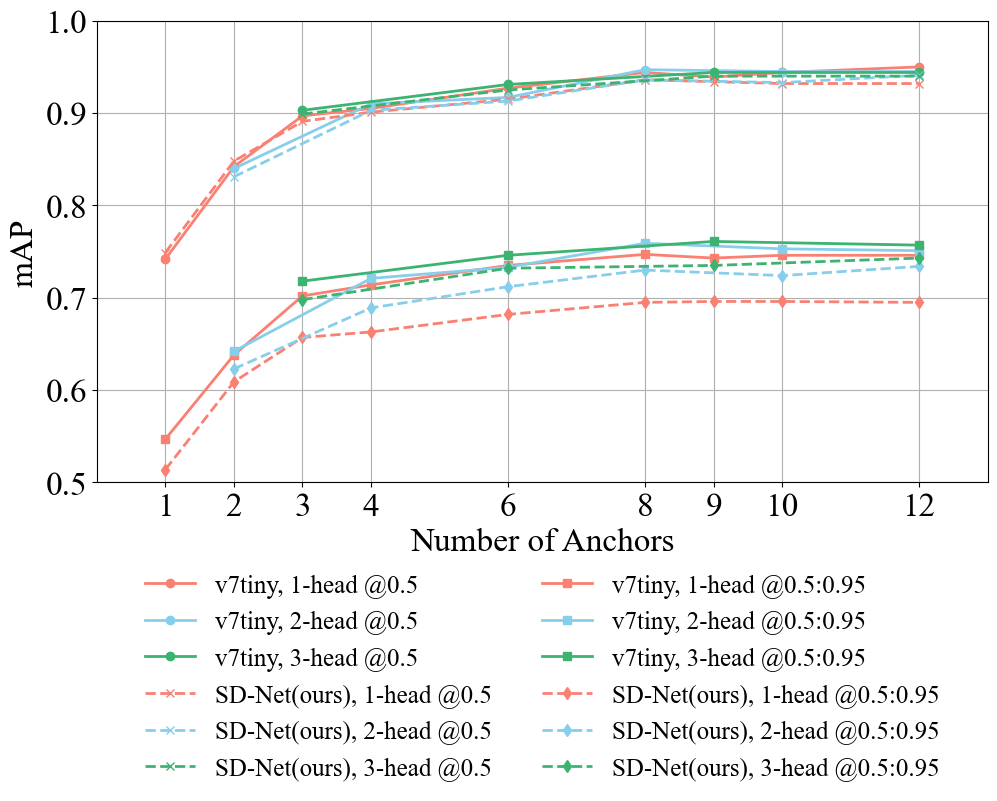
\includegraphics[width=\columnwidth]{figures/fig_08.png}}
    \caption{(Top) mAP@0.5 and (Bottom) mAP@0.5:0.95 results for the baseline Yolov7-tiny and the proposed SD-Net model, evaluated with varying numbers of detection heads and anchor boxes. As the number of anchor boxes increases, mAP generally improves; however, the performance gains tend to plateau at higher anchor box counts. Increasing the number of heads leads to noticeable improvements in mAP@0.5:0.95, while its effect on mAP@0.5 is relatively marginal.}
    \label{fig:map_results}
\end{figure}

A noteworthy finding is that the proposed \ac{SD-Net} model achieves comparable or even superior performance to YOLOv7-tiny despite using significantly fewer parameters. For example, in some configurations such as the 1-head 1-anchor and 1-head 2-anchor models, the \ac{SD-Net} model outperforms the baseline in mAP@0.5. Although the difference becomes apparent in mAP@0.5:0.95, the primary goal of this system is to detect whether a passenger is descending the stairs, for which mAP@0.5 is a more suitable metric. Therefore, the \ac{SD-Net} model's comparable performance on mAP@0.5 demonstrates that it successfully retains high accuracy for its core task.

As shown in Table~\ref{tab:full_comparison}, the mAP@0.5 of the YOLOv7-tiny 3-head 9-anchor model is 94.4\%, while that 
of the \ac{SD-Net} 1-head 8-anchor model is 93.6\%, a marginal difference of only 0.8\%. However, the \ac{SD-Net} model reduces the number of heads by two and anchor boxes by one, cutting the parameter count by over 80.9\% (from 6.02 M to 1.15 M). This reduction also leads to a 45.7\% improvement in inference speed (from 1.451 ms to 0.788 ms). Thus, depending on deployment requirements, the proposed model can be preferable. For instance, in systems designed to assist train engineers by detecting passengers on stairs and recommending optimal door-closing times—or warning passengers about risky behavior—the \ac{SD-Net} model’s lightweight architecture and fast inference could be highly beneficial.

% Moreover, introducing new systems or security mechanisms often 
% faces delays due to integration challenges, compatibility 
% issues with existing infrastructure, and inter-departmental 
% coordination. In such cases, the proposed model – being 
% extremely lightweight and computationally efficient - can be 
% effectively implemented as a standalone system on edge devices, 
% avoiding interference with existing operations.

Fig.~\ref{fig:inference_results} presents the inference times of all 38 models with the number of anchor boxes on the $x$-axis and the inference time on the $y$-axis. It is clearly observed that inference time increases with the number of detection heads. A significant difference is also noted between the baseline YOLOv7-tiny models and the proposed \ac{SD-Net} models—all \ac{SD-Net} models demonstrate significantly faster inference speeds under the same number of heads. This is attributed to the lightweight architecture of the \ac{SD-Net} model, which results in a drastically reduced parameter count. However, within a fixed number of heads, increasing the number of anchor boxes does not significantly affect inference time. Although more anchors lead to slightly larger output vectors at each grid cell, the additional computation is negligible compared to overall network inference time. In other words, the added overhead from anchor boxes at the output stage has minimal impact on total inference performance.

\begin{figure}[!b]
    \centerline{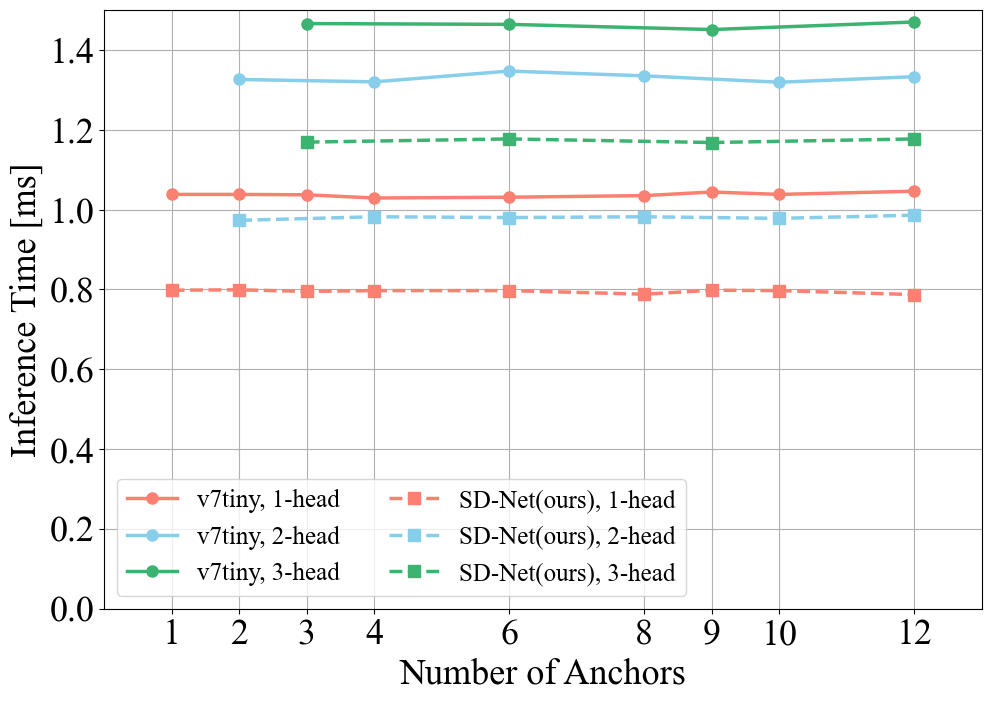
\includegraphics[width=\columnwidth]{figures/fig_09.png}}
    \caption{Inference time comparison for 38 different models.}
    \label{fig:inference_results}
\end{figure}


\section{Discussion}
% The proposed \ac{SD-Net} model holds significant practical value for real-world subway systems. One feasible deployment strategy involves installing standalone edge-camera at each stairway on the platform. This strategy is practical because the system can operate independently, without connecting to complex, existing train control systems. This edge-based system can be applied in three primary ways: (1) providing immediate alarms to conductors in manual systems, (2) enabling optimal door-closing timing in automated systems, or (3) issuing direct warnings to passengers on the platform. Therefore, for deployment in resource-constrained environments such as these edge devices, inference speed and model compactness are more critical design objectives than marginal gains in accuracy. This demonstrates that \ac{SD-Net} is a superior and more realistic solution for practical deployment than heavier general purposed baseline models.

The proposed \ac{SD-Net} model holds significant practical value for real-world subway systems. One feasible deployment strategy involves installing standalone edge cameras at each stairway on the platform. This strategy is practical because the system can operate independently, without connecting to complex, existing train control systems. This edge-based system can be applied in three primary ways: (1) providing immediate alarms to conductors in manual systems, (2) enabling optimal door-closing timing in automated systems, or (3) issuing direct warnings to passengers on the platform. Therefore, for deployment in resource-constrained environments such as these edge devices, inference speed and model compactness are more critical design objectives than marginal gains in accuracy. This demonstrates that \ac{SD-Net} is a superior and more realistic solution for practical deployment than heavier general-purpose baseline models.

% While the model's bounding boxes are less precise at stricter \ac{IoU} thresholds (\ac{mAP}@0.5:0.95), this is acceptable. 
% The system's primary goal is rapid presence detection—to quickly identify if a passenger is descending—not perfect localization. For this warning application, a 'good enough' detection 
% (\ac{IoU} $> 0.5$) is sufficient, making \ac{mAP}@0.5 the more 
% representative performance metric.

While the model's bounding boxes are less precise at stricter \ac{IoU} thresholds (\ac{mAP}@0.5:0.95), this is acceptable. 
The system's primary goal is rapid presence detection—to quickly identify if a passenger is descending—not perfect localization. For this warning application, a sufficient detection (\ac{IoU} $> 0.5$) is considered adequate, making \ac{mAP}@0.5 the more representative performance metric.

We trained and tested it on a dataset from only one station and one fixed camera. While the platform structure at most stations involves passengers arriving by descending stairs, this specialization is a clear limitation. The model's performance remains unverified for other stations, varying camera angles, different access routes like elevators or transfer passages, or during high-density rush hour conditions.

Furthermore, the proposed \ac{SD-Net} is not a standalone accident prevention system but rather a core input module for practical system integration. It is designed to function as the visual sensing component of a complete safety system. For this model to be operationally effective, it requires integration with additional components that can interpret its output. This includes a module for tracking passenger trajectory and speed, which would use the continuous detections from \ac{SD-Net} to estimate a passenger's velocity. This data, combined with a behavioral model that infers boarding intent from a descending passenger, would feed a risk-prediction algorithm. This algorithm would then calculate if the passenger can safely reach the door before door closure, ultimately transmitting a final 'wait' or 'close' judgment to a conductor's
monitor (or door control unit computer) or a passenger-facing warning system.


\section{Conclusion}
This study presented the Safe Door Network (\ac{SD-Net}), a 
task-specific object detection framework tailored to prevent 
passenger door accidents by detecting human behavior 
indicative of imminent boarding attempts. By redesigning the 
\ac{YOLO}v7-tiny baseline with a \ac{PFL}-based backbone and 
optimizing the detection head and anchor box configurations, 
we achieved a practical optimum in the accuracy-efficiency 
trade-off.

Experimental results show that the proposed \ac{SD-Net} model 
(1-head, 8-anchor) exhibits only a marginal 0.8\% difference 
in \ac{mAP}@0.5 compared to the \ac{YOLO}v7-tiny model 
(3-head, 9-anchor) (94.4\% vs. 93.6\%). In exchange, the 
\ac{SD-Net} model drastically reduces the parameter count by 
over 80.9\% and improves inference speed by 45.7\%.

In conclusion, the compact size and real-time performance of 
the \ac{SD-Net} model make it highly suitable for deployment 
on embedded systems at station platforms, proactively providing early warnings to train conductors, decision 
support for automated door control systems, or real-time alerts to passengers at risk.

Future work will focus on generalizing the \ac{SD-Net} model and integrating it into a complete proactive safety framework. 
Generalization involves expanding the dataset to include diverse station layouts, camera angles, and passenger densities. 
Integration will focus on developing a module for tracking passenger trajectory and speed, which will feed a 
risk-prediction algorithm. This algorithm will calculate safe door-closing times, enabling the system to 
transmit a final judgment to a conductor's monitor, an automated door control unit, or a passenger-facing warning system.

\bibliography{references}
\bibliographystyle{IEEEtran}

\begin{IEEEbiography}[{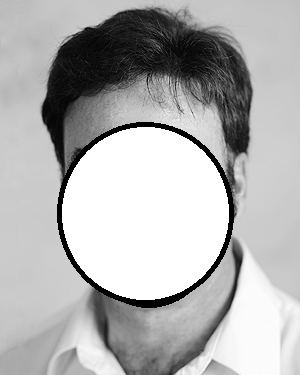
\includegraphics[width=1in,height=1.25in,clip,keepaspectratio]{figures/a1.png}}]{First A. Author} (M'76--SM'81--F'87) and all authors may include 
biographies. Biographies are often not included in conference-related
papers. This author became a Member (M) of IEEE in 1976, a Senior
Member (SM) in 1981, and a Fellow (F) in 1987. The first paragraph may
contain a place and/or date of birth (list place, then date). Next,
the author's educational background is listed. The degrees should be
listed with type of degree in what field, which institution, city,
state, and country, and year the degree was earned. The author's major
field of study should be lower-cased. 

The second paragraph uses the pronoun of the person (he or she) and not the 
author's last name. It lists military and work experience, including summer 
and fellowship jobs. Job titles are capitalized. The current job must have a 
location; previous positions may be listed 
without one. Information concerning previous publications may be included. 
Try not to list more than three books or published articles. The format for 
listing publishers of a book within the biography is: title of book 
(publisher name, year) similar to a reference. Current and previous research 
interests end the paragraph. The third paragraph begins with the author's 
title and last name (e.g., Dr.\ Smith, Prof.\ Jones, Mr.\ Kajor, Ms.\ Hunter). 
List any memberships in professional societies other than the IEEE. Finally, 
list any awards and work for IEEE committees and publications. If a 
photograph is provided, it should be of good quality, and 
professional-looking. Following are two examples of an author's biography.
\end{IEEEbiography}

\begin{IEEEbiography}[{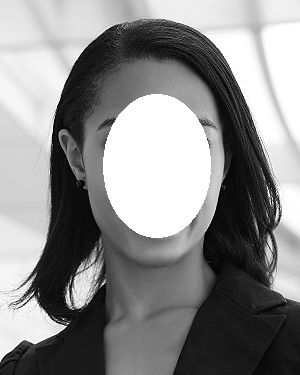
\includegraphics[width=1in,height=1.25in,clip,keepaspectratio]{figures/a2.png}}]{Second B. Author} was born in Greenwich Village, New York, NY, USA in 
1977. He received the B.S. and M.S. degrees in aerospace engineering from 
the University of Virginia, Charlottesville, in 2001 and the Ph.D. degree in 
mechanical engineering from Drexel University, Philadelphia, PA, in 2008.

From 2001 to 2004, he was a Research Assistant with the Princeton Plasma 
Physics Laboratory. Since 2009, he has been an Assistant Professor with the 
Mechanical Engineering Department, Texas A{\&}M University, College Station. 
He is the author of three books, more than 150 articles, and more than 70 
inventions. His research interests include high-pressure and high-density 
nonthermal plasma discharge processes and applications, microscale plasma 
discharges, discharges in liquids, spectroscopic diagnostics, plasma 
propulsion, and innovation plasma applications. He is an Associate Editor of 
the journal \emph{Earth, Moon, Planets}, and holds two patents. 

Dr. Author was a recipient of the International Association of Geomagnetism 
and Aeronomy Young Scientist Award for Excellence in 2008, and the IEEE 
Electromagnetic Compatibility Society Best Symposium Paper Award in 2011. 
\end{IEEEbiography}

\begin{IEEEbiography}[{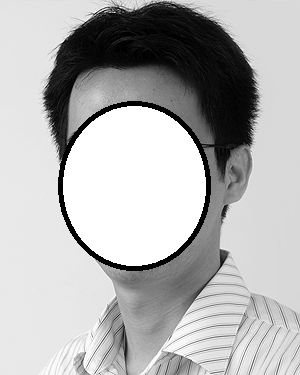
\includegraphics[width=1in,height=1.25in,clip,keepaspectratio]{figures/a3.png}}]{Third C. Author, Jr.} (M'87) received the B.S. degree in mechanical 
engineering from National Chung Cheng University, Chiayi, Taiwan, in 2004 
and the M.S. degree in mechanical engineering from National Tsing Hua 
University, Hsinchu, Taiwan, in 2006. He is currently pursuing the Ph.D. 
degree in mechanical engineering at Texas A{\&}M University, College 
Station, TX, USA.

From 2008 to 2009, he was a Research Assistant with the Institute of 
Physics, Academia Sinica, Tapei, Taiwan. His research interest includes the 
development of surface processing and biological/medical treatment 
techniques using nonthermal atmospheric pressure plasmas, fundamental study 
of plasma sources, and fabrication of micro- or nanostructured surfaces. 

Mr. Author's awards and honors include the Frew Fellowship (Australian 
Academy of Science), the I. I. Rabi Prize (APS), the European Frequency and 
Time Forum Award, the Carl Zeiss Research Award, the William F. Meggers 
Award and the Adolph Lomb Medal (OSA).
\end{IEEEbiography}

\end{document}
